\documentclass[lettersize,journal]{IEEEtran}
% Essential packages
\usepackage[utf8]{inputenc}
\usepackage{amsmath,amssymb,amsfonts,empheq}
\usepackage{graphicx}
\usepackage{textcomp}
\usepackage{url}
\usepackage{verbatim}
\usepackage{array}
\usepackage{rotating}
\usepackage{stfloats}
\usepackage{cite}
\usepackage{soul}
\usepackage[margin=2cm]{geometry}
\usepackage{colortbl}
% Algorithm packages
\usepackage{algorithm}
\usepackage{algorithmic}

% Subfigures
\usepackage[caption=false,font=normalsize,labelfont=sf,textfont=sf]{subfig}

% MATLAB code formatting
\usepackage{matlab-prettifier}

% Hyperlinks and references
\usepackage{hyperref}
\usepackage{cleveref}

% Adjust box
\usepackage{adjustbox}

% Custom math operators
\DeclareMathOperator{\sgn}{sgn}
\DeclareMathOperator{\sat}{sat}
\DeclareMathOperator{\gsgn}{gsgn}
\DeclareMathOperator{\gsat}{gsat}
\DeclareMathOperator{\for}{for}
\DeclareMathOperator{\diag}{diag}
\DeclareMathOperator{\var}{var}
\DeclareMathOperator{\limit}{limit}
\DeclareMathOperator{\SNR}{SNR}
\DeclareMathOperator{\rad}{rad}
\DeclareMathOperator{\eig}{eig}
\DeclareMathOperator{\s}{s}
\DeclareMathOperator{\LF}{LF}
\DeclareMathOperator{\sgnsingle}{sgn}
\DeclareMathOperator{\sgnset}{\overline{sgn}}
\DeclareMathOperator{\proj}{proj}

% Cleveref name formats
\crefname{equation}{}{}
\Crefname{figure}{Fig.}{Figs.}
\crefname{section}{Sec.}{Secs.}
\crefname{table}{Table}{Tables}

% Theorem environments
\newtheorem{theorem}{Theorem}
\newtheorem{lemma}{Lemma}
\newtheorem{proposition}{Proposition}
\newtheorem{remark}{Remark}
\newtheorem{definition}{Definition}
\newtheorem{corollary}{Corollary}
\newtheorem{example}{Example}


\hyphenation{op-tical net-works semi-conduc-tor IEEE-Xplore}
% updated with editorial comments 8/9/2021

\begin{document}

\title{Control of resonance-based fatigue testing  machines}

\author{Mohammad Rasool MOJALLIZADEH, Benoît PICHEREAU, and Etienne PESSARD
        % <-this % stops a space
\thanks{The authors are with the Arts et Métiers Institute of Technology, LAMPA, F-49035 Angers, France (e-mails: \{mohammad-rasool.mojallizadeh, etienne.pessard, benoit.pichereau\} @ ensam.eu)}
\thanks{Corresponding author: Mohammad Rasool MOJALLIZADEH}
}

% The paper headers
\markboth{IEEE Transactions on Control Systems Technology}%
{MOJALLIZADEH \MakeLowercase{\textit{et al.}}: Control of resonance-based fatigue testing machines}

%\IEEEpubid{0000--0000/00\$00.00~\copyright~2021 IEEE}
% Remember, if you use this you must call \IEEEpubidadjcol in the second
% column for its text to clear the IEEEpubid mark.

\maketitle

\begin{abstract}
This work investigates the design of controllers for resonance-based fatigue testing machines. Unlike conventional systems, resonance-based machines require smaller setups, consume less energy, and significantly reduce test duration by maintaining the specimen at its natural excitation frequency. Achieving this requires a robust control system capable of driving the system to its resonance frequency while rejecting disturbances such as temperature variations and unmodeled dynamics—particularly those caused by crack formation, which alters the specimen’s properties, including its resonance frequency, during testing. A tutorial-style review of state-of-the-art control systems developed for resonance-based fatigue machines is presented in terms of the resonance frequency and displacement tracking. Various control design techniques are discussed for these models, including proportional-integral-derivative (PID) and fuzzy controllers. Subsequently, a control-oriented model is developed using an identification method, which is essential for any model-based controller design. However, this model is subject to uncertainties and perturbations, making control design more challenging. To address this, a sliding-mode controller (SMC) based on the twisting algorithm is proposed to ensure robust stability. Comparative analyses using both numerical simulations and experimental results demonstrate the advantages of the proposed twisting controller over conventional controllers, namely PI and fuzzy controllers.
\end{abstract}

\begin{IEEEkeywords}
Resonance-based fatigue testing, control design, identification, sliding-mode control, twisting controller
\end{IEEEkeywords}

\section{Introduction} \label{S_introduction}
\IEEEPARstart{F}{atigue}
analysis plays a crucial role in designing durable and long-lasting components, helping to prevent unexpected failures and enhance overall safety. Experimental fatigue testing has been used since the 19th century \cite{radaj2007ermudungsfestigkeit}.
 The design of fatigue-loaded structures is often based on the concept of an endurance limit (at 1E6 or 1E7 cycles), defined as the maximum load below which a structure is assumed to have an infinite lifetime. However, many studies have shown that some materials and structures do not exhibit a clear endurance limit, making its existence a matter of debate. Consequently, the reliable characterization of fatigue resistance at very high cycle numbers ($\geq$ 1E7 cycles), using rapid and energy-efficient testing methods, remains an open problem. To address these challenges, resonance-based fatigue testing machines have been developed. These machines apply dynamic load cycles near the specimen’s resonance frequency (i.e., the material under investigation), which significantly reduces power consumption. Moreover, since the resonance frequency is generally high, the required number of load cycles can be completed in a much shorter time compared to traditional fatigue testing methods. Resonance-based fatigue testing machines are designed with various architectures to accommodate a wide range of materials and structures, both at reduced and real scales. These include applications in concrete \cite{SCHRAMM2024117045}, railroad rails \cite{SCHNEIDER2018171,herrmann2018simulation_Thesis}, pipes \cite{Santus_2024}, packaging \cite{Rouillard_2000}, and electronic PCB boards \cite{DORANGA2024115368,ikehara2010development}.

One method for testing large-scale structures involves using imbalance motors mounted on tension springs to excite concrete specimens \cite{SCHRAMM2024117045}, as well as axially loaded components such as railroad rails \cite{SCHNEIDER2018171,herrmann2018simulation_Thesis} and pipes \cite{Santus_2024}. In these studies, the resonance frequency is determined offline using finite element methods (FEM) and manually set by the user. However, this approach does not account for automatic resonance frequency tracking, which can vary during testing and lead to performance degradation. To address synchronization and frequency tracking, a time-clocked state machine combined with a PI controller is employed \cite{SCHRAMM2024117045,SCHNEIDER2018171,herrmann2018simulation_Thesis}. According to \cite{SCHNEIDER2018171}, operating near the resonance frequency can cause closed-loop instability; therefore, the excitation frequency is typically maintained at 90\% of the resonance frequency. Alternative resonance-based fatigue testing systems utilize electrodynamic \cite{Su2014,George_2006,CESNIK20125370,gautrelet2020resonance,DORANGA2024115368,Rouillard_2000}, electro-hydraulic\footnote{PLG-100 is a commercial fatigue testing machine based on electro-hydraulic shakers \cite{met11101512}.} \cite{Ji_2010,Rouillard_2000}, or ultrasonic shakers \cite{Stanzl01041980_fast_ultrasonic}. These systems are generally applied to reduced-scale specimens, such as stainless steel samples \cite{Gautrelet_2020}, electronic boards \cite{Su2014,feng2003development_Japaneese}, and packaging components \cite{Rouillard_2000}. Additionally, multi-axial fatigue testing has been demonstrated using these shaker technologies \cite{George_2006,Dupke2026}.

Developing an efficient resonance-based fatigue testing machine requires a control system that fulfills two primary objectives: (1) maintaining the excitation frequency close to the specimen’s resonance frequency to reduce the required energy, and (2) achieving the target displacement or force amplitude without exceeding it to comply with standards such as DIN 50100 \cite{DIN_standard}. Despite the importance of such a control system, this aspect is often overlooked in the literature, where instrumentation is typically described without detailing the underlying control algorithms. Motivated by this gap, the present work provides a comprehensive literature review on control strategies for resonance-based fatigue testing machines. The objective is to characterize the properties of existing approaches and identify research gaps stemming from the limited focus on control system design. To this end, a control-oriented model of the system is developed using system identification techniques. Based on this model, a sliding mode control (SMC) strategy is proposed using the twisting algorithm to ensure robust closed-loop stability. SMC is a well-established control methodology (see \cite{Slotine1991} for an introduction), extensively studied since 1955 \cite{Utkin1955}, and valued for its finite-time convergence and robustness to disturbances. Among the various SMC techniques, the twisting controller (TC) \cite{UTKIN2020_higher_order, Orlov_twisting, Utkin_twisting, POLYAKOV_twisting, Santiesteban_twisting, TORRESGONZALEZ2017_twisting, Santiesteban_twisting} is recognized as a second-generation higher-order sliding mode algorithm, as classified in \cite{Fridman2015}.


Numerical simulations and realistic experiments are conducted to evaluate the performance of the proposed control system and to compare it with conventional controllers, such as PI and fuzzy controllers. Based on these results, future perspectives are discussed to address existing limitations and advance toward more efficient control strategies. The remainder of the manuscript is organized as follows. In \Cref{S_control_system}, a tutorial-style review of control systems developed for resonance-based fatigue testing machines is presented. \Cref{S_SMC} introduces a control-oriented mathematical model derived using system identification methods, followed by the development of a sliding mode control system based on the twisting algorithm to ensure robust stability. Numerical simulations and experimental validations are provided in \Cref{S_simulations} and \Cref{S_experiments}, respectively, to quantify performance and enable comparative analysis. Finally, \Cref{S_conclusions} concludes the work and outlines future research directions. The nomenclature and the mathematical notation used in the manuscript is explained in \Cref{T_nomenclature,T_notation}, respectively.



\begin{table}[h]
    \centering
    \begin{tabular}{|c|l|}
        \hline
        \textbf{Abbreviation} & \textbf{Definition} \\ \hline
        SMC & Sliding Mode Control \\ \hline
        TC & Twisting Controller \\ \hline
        PID & Proportional-Integral-Derivative \\ \hline
        PI & Proportional-Integral \\ \hline
        FEM & Finite Element Method \\ \hline
        PLL & Phase-Locked Loop \\ \hline
        LF & Low-Pass Filter \\ \hline
        DIN & Deutsches Institut für Normung \\ \hline
    \end{tabular}
    \vspace{0.1cm}
    \caption{Nomenclature of abbreviations used in the manuscript}
    \label{T_nomenclature}
\end{table}

\begin{table}[h]
    \centering
    \begin{tabular}{|l|}
        \hline
        $t$: continuous-time variable \\
	 $k$: discrete-time variable \\ 
        $K$:  stiffness coefficient \\
	 $m$:  mass of the system \\
        $b$:  damping coefficient \\
        $x_1$:  specimen displacement,  $x_2$  specimen velocity \\
        $f$:  excitation force applied by the shaker \\
        $s$:  laplace transform variable \\
        $\omega_0$:  natural frequency of the system \\
        $\omega_d$:  damped (resonance) resonance frequency,
        $\zeta$:  damping ratio \\
        $\phi$:  phase difference between two accelerometers  \\
        $\phi_d$:  desired phase (typically $\pi/2$) \\
        $\theta$:  cosine of the phase $\phi$ \\
        $a$:  amplitude of the excitation force \\
        $a_d$:  desired displacement amplitude \\
        $u_1$: control input for excitation frequency \\
        $u_2$:  control input for excitation amplitude \\
        $z_1$, $z_2$:  state variables in the identified phase tracking model \\
        $e_1$, $e_2$:  error states in the amplitude tracking model \\
$X_1$: Laplace transformation of $x_1$ \\
$X_2$: Laplace transformation of $x_2$ \\
$F$: Laplace transformation of $f$ \\
$Z^{-1}$: unit delay operator \\
$k_p$, $k_d$, $k_i$: proportional, derivative, and integral gains of the PID\\
$\alpha_1$, $\alpha_2$, $\alpha_3$: parameters of the fuzzy controller \\
$x_{1h}$ and $x_{1p}$: homogeneous and particular solutions of $x_1$ \\
$\gamma$: a positive real constant \\
$p$ and $q$: parameters of the identified model \\
$\bar{p}$ and $\bar{q}$: nominal values of $p$ and $q$, respectively \\
$\tilde{p}$ and $\tilde{q}$: uncertain (unknown) parts of $p$ and $q$, respectively \\
$b_1$ and $b_2$: parameters of the twisting controller \\
$k_m$, $k_M$, $k_a$: bounds of the identified parameters \\
$z_1$ and $z_2$: state variables of the phase error system \\
$e_1$ and $e_2$: state variables of the displacement error system \\
$J_x$: displacement tracking cost function \\
 $J_\phi$: phase tracking cost function \\
$J$: total cost function \\
$\lambda$: selection of the set-valued signum function \\
$q_1$, $q_2$: two intermediate terms used in $\lambda$ \\
\hline
    \end{tabular}
    \vspace{0.1cm}
    \caption{Mathematical notation used in the manuscript}
    \label{T_notation}
\end{table}


\section{Review of the control systems developed for resonance-based fatigue testing machines} \label{S_control_system}

The block diagram of a typical resonance-based fatigue testing machines is shown in \Cref{F_control_diagram}. A shaker is employed to apply dynamic loads in order to excite the structure at its resonance frequency and achieve the desired displacement or force in certain cases. Since the resonance frequency is either unknown or only approximately known—and may vary over time during testing—a mechanism for resonance frequency search and tracking is essential. The methods for resonance frequency tracking and displacement control are discussed in \Cref{S_frequency_seeking} and \Cref{S_amplitude_tracking}, respectively. Finally, the instrumentation and hardware implementations reported in the literature for realizing such control systems are reviewed in \Cref{S_instrumentation}.
\begin{figure}
    \centering    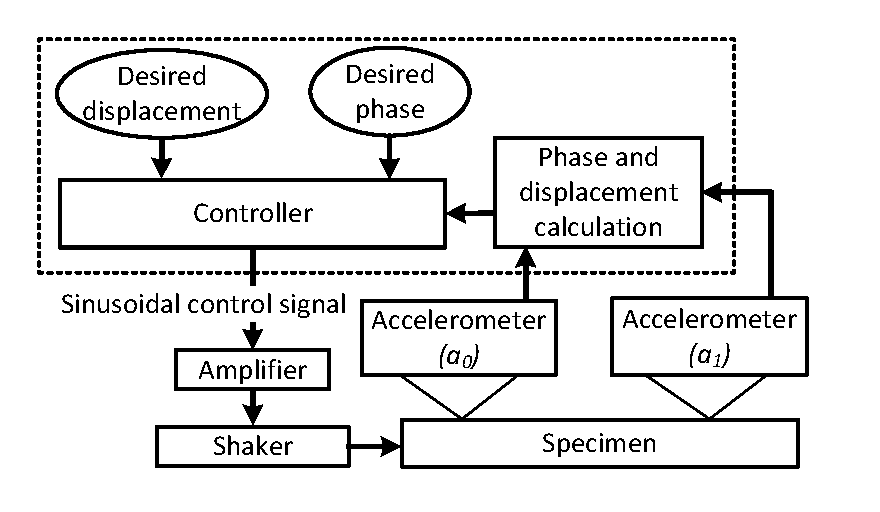
\includegraphics[width=\linewidth]{Control_system_fatigue_total.pdf}
    \caption{Closed-loop Control system in resonance-based fatigue testing machines based on shakers}
    \label{F_control_diagram}
\end{figure}



\subsection{Frequency seeking and tracking}  \label{S_frequency_seeking}


The specimen’s resonance frequency is an unknown and time-varying parameter during fatigue testing, influenced by factors such as temperature changes, damage and crack propagation. Therefore, implementing a resonance tracking mechanism is essential. As illustrated in \Cref{F_control_diagram}, two accelerometers are typically used to measure the specimen’s deformation, and the phase difference between these signals is computed using a phase detection block (see \Cref{S_phase_detection}). According to the modeling approach described in \Cref{S_resonance_modeling}, maintaining a specific phase difference—typically 90 degrees—between the two signals ensures operation at the resonance frequency. The measured and desired phase values are then given to a frequency controller, which generates the control frequency. This process is commonly referred to as {\em track and dwell} or a phase-locked loop (PLL) implementation. The modeling of the resonance dynamics is detailed in \Cref{S_resonance_modeling}, and the frequency tracking controllers reported in the literature are reviewed in \Cref{S_frequency_controller}.



\subsubsection{Modeling of the resonance dynamics} \label{S_resonance_modeling}

Regardless of the structural configurations reviewed in \Cref{S_introduction}, the dynamic behavior of resonance-based fatigue testing machines can generally be modeled as a second-order linear system. This modeling approach is supported by previous studies involving imbalance motors \cite{SCHNEIDER2018171,herrmann2018simulation_Thesis,SCHRAMM2024117045}, electrodynamic shakers \cite{feng2003development_Japaneese}, and electro-hydraulic actuators \cite{Ji_2010}.
\begin{subequations}
  \begin{empheq}[left=\empheqlbrace]{align}
\dot{x}_1(t)&=x_2(t) \label{E_plant_1} \\
\dot{x}_2(t)&=\frac{1}{m} \big ( -Kx_1(t)-bx_2(t)+f(t)  \big) ,\label{E_plant_2} 
  \end{empheq}
\label{E_plant_no_output}
\end{subequations}
where $t$ is the continuous-time variable (which may be omitted for brevity), $x_1$ and $x_2$ represent the specimen’s displacement and velocity, respectively; $f$ is the sinusoidal excitation force generated by the shaker; $K$ and $b$ are the stiffness and damping coefficients; and $m$ is the mass of the system. The objective is to compute and apply the excitation force $f$ such that the system operates at resonance. Applying the Laplace transform to \Cref{E_plant_no_output} yields the following transfer function:
\begin{equation}
\frac{X_1(s)}{F(s)} = \frac{1}{ms^2 + bs + K},
\label{E_Laplace}
\end{equation}
where $X_1(s)$ and $F(s)$ are the Laplace transforms of $x_1(t)$ and $f(t)$, respectively, and $s$ is the Laplace variable. This transfer function can be rewritten in the standard second-order form as:
\begin{subequations}
  \begin{empheq}[left=\empheqlbrace]{align}
\frac{X_1(s)}{F(s)}&=\frac{\frac{1}{m}}{s^2+2\zeta \omega_0 s+\omega_0^2} \label{E_TF_standard_1}  \\ 
\omega_0&=\sqrt{\frac{k}{m}} \label{E_TF_standard_2}  \\ 
\omega_d&=\omega_0 \sqrt{1-\zeta^2}, \label{E_TF_standard_3} \\
\zeta&=\frac{b}{2\sqrt{km}}, \label{E_TF_standard_4}
  \end{empheq}
\label{E_TF_standard}
\end{subequations}
where $\omega_0$ is the natural angular frequency, $\zeta$ is the damping ratio, and $\omega_d$ is the resonance (damping) frequency. The bode diagram of \Cref{E_TF_standard} for the parameters $m=0.01772$~kg, $k=256$~N/m, and $b=0.1$~N.s/m is shown in \Cref{F_Bode} leading to the resonance frequency $\omega_d \simeq 39$~rad/s. As can be seen, at $\omega_d$, the transfer function amplitude \Cref{E_TF_standard_1} is maximized, meaning that to maximize the transferred energy and minimize the dissipation, the input force must be in the sinusoidal form with the frequency $\omega=\omega_d$ as follows:
\begin{equation}
f(t)=a\sin(\omega t),
\label{E_F_resonance}
\end{equation}
where $a$ denotes the amplitude of the force generated by the actuator (shaker). However, since $\omega_d$ is only approximately known and varies over time in practice, generating the excitation force using \Cref{E_F_resonance} is impractical. To address this limitation, rather than relying on such an open-loop control law, phase-tracking closed-loop control strategies are employed in the literature, as discussed in \Cref{S_frequency_controller}.

\begin{figure}
    \centering    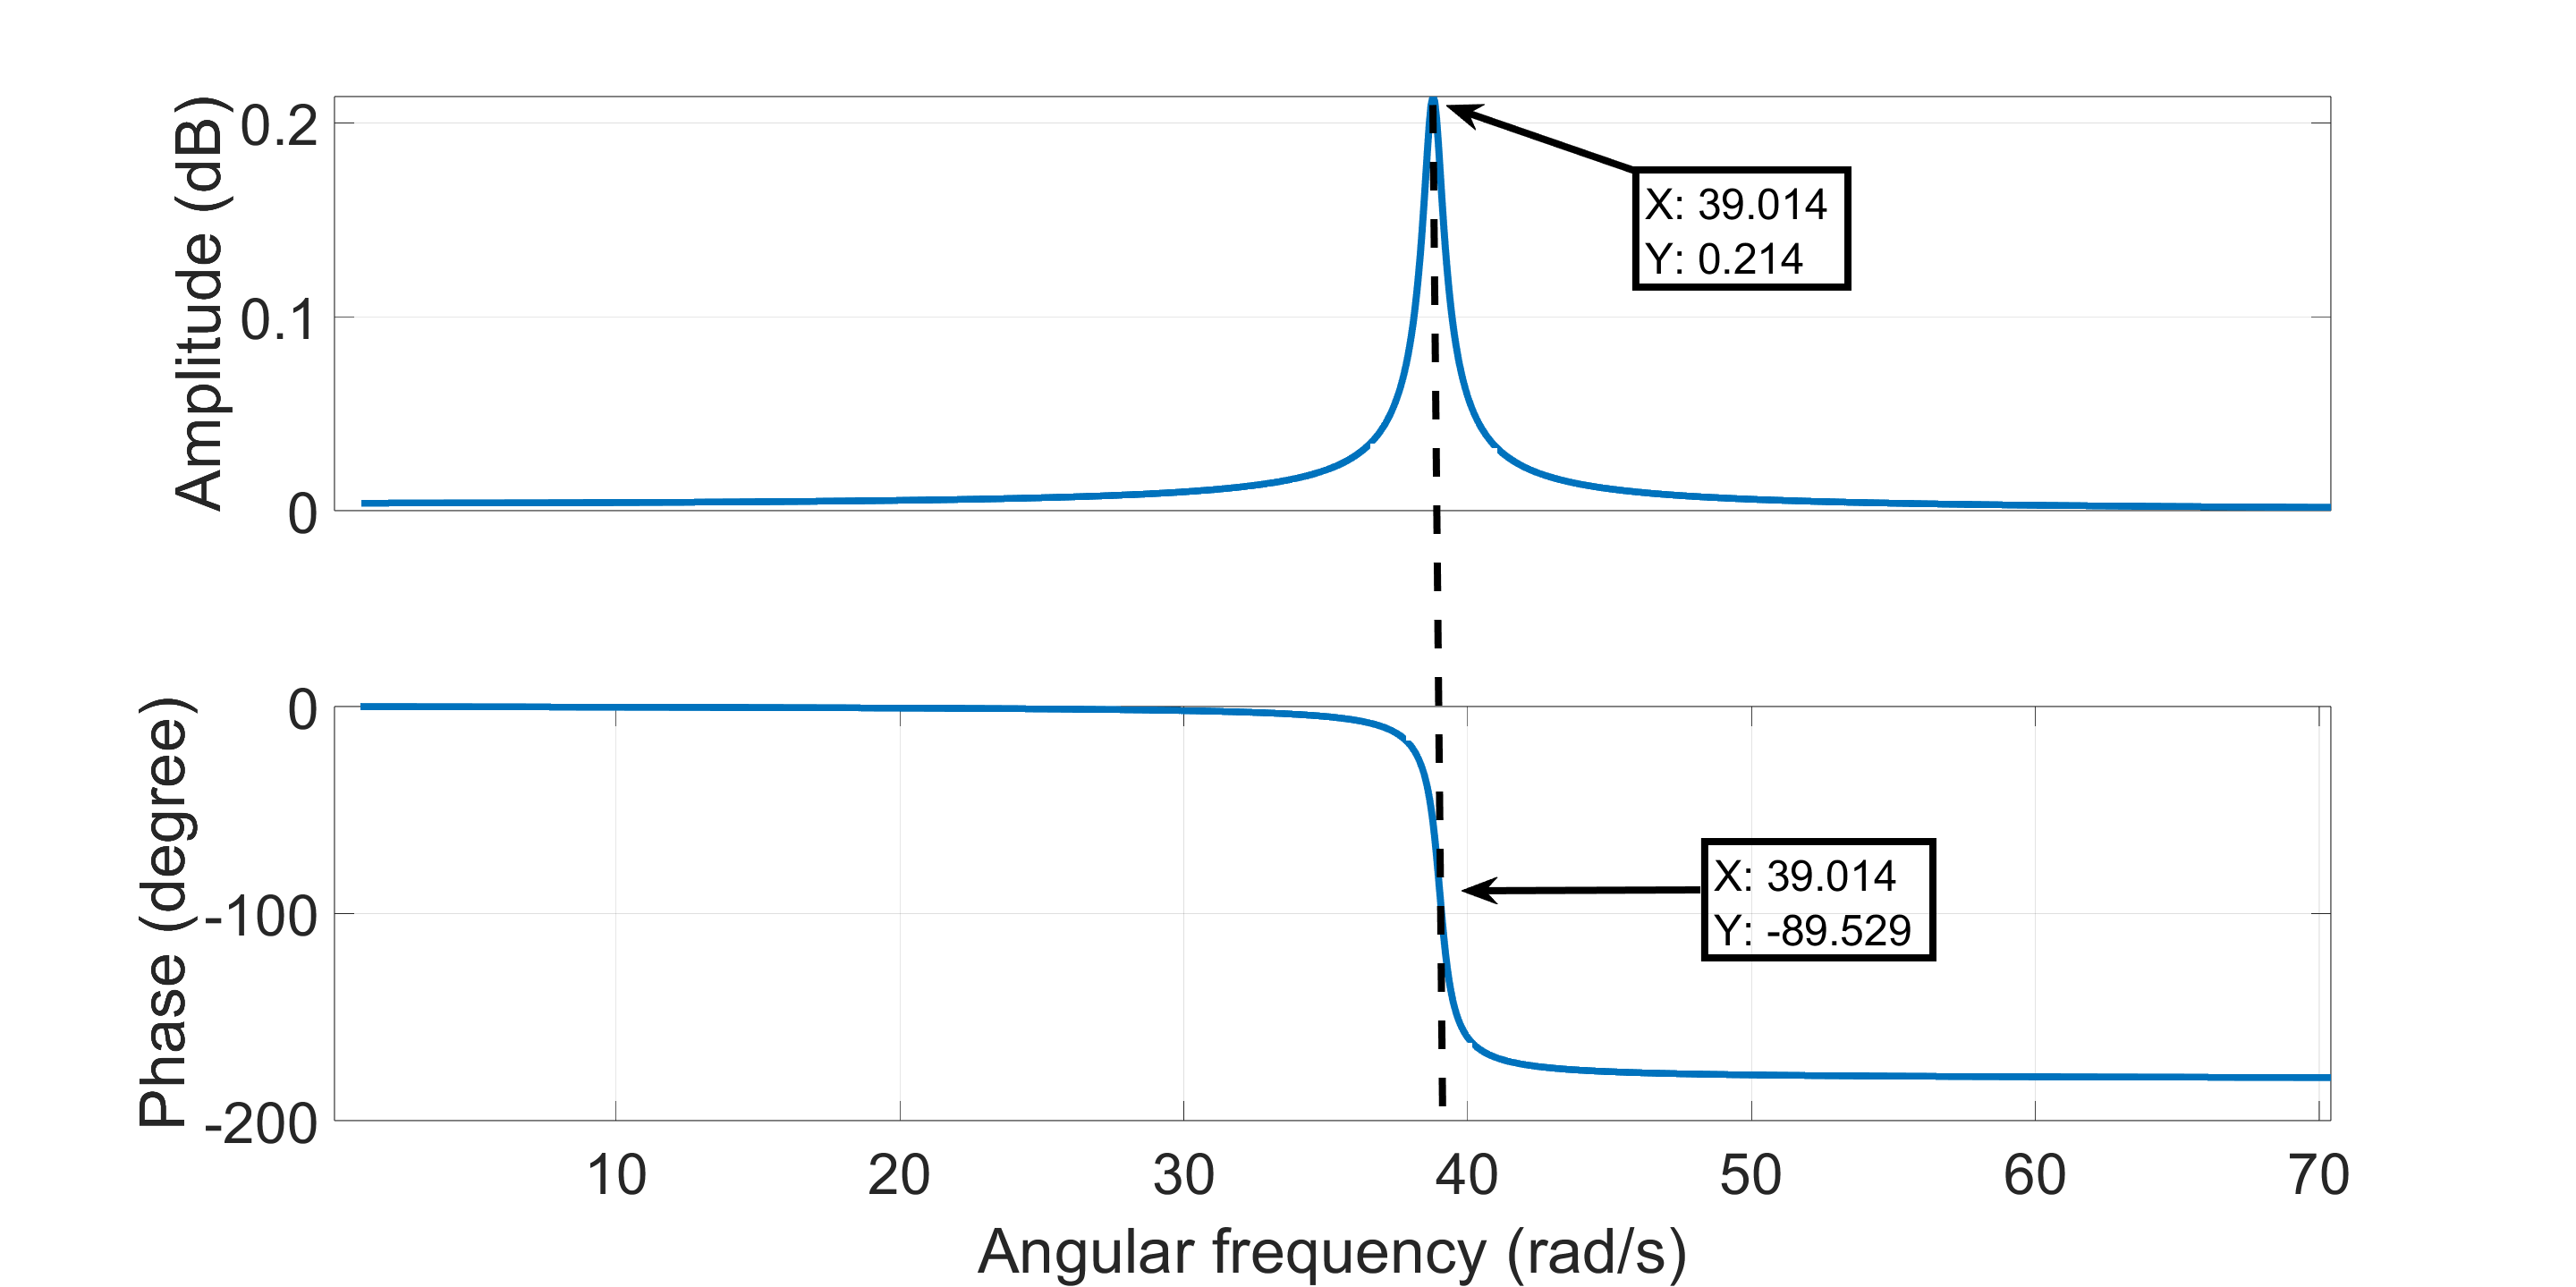
\includegraphics[width=\linewidth]{F_bode.png}
    \caption{Bode diagram of the resonance dynamics for the parameters $m=0.01772$~kg, $k=256$~N/m, and $b=0.12$~Ns/m}
    \label{F_Bode}
\end{figure}




\subsubsection{Phase tracking controller} \label{S_frequency_controller}


Assuming that the specimen resonance frequency $\omega_d$ is known, one may use \Cref{E_F_resonance} to generate the excitation force \cite{SCHNEIDER2018171,herrmann2018simulation_Thesis,SCHRAMM2024117045}. However, $\omega_d$ is typically estimated using FEM-based numerical simulations, which may not accurately reflect real-world conditions. Moreover, $\omega_d$ can vary over time. Therefore, a closed-loop control strategy is required to continuously track the resonance frequency. Such a control strategy is commonly referred to as a PLL. As illustrated in \Cref{F_Bode}, the amplitude of the transfer function in \Cref{E_Laplace} reaches its maximum when the phase difference between the input force and the output displacement is approximately $90^\circ$ (exactly $90^\circ$ for $\zeta = 0$). Despite its importance, many studies in this area do not detail the controller used in the frequency tracking block \cite{Gautrelet_2020}, leaving the specific control strategies unclear. According to \Cref{T_frequency_seeking}, two types of controllers—namely, PI and fuzzy controllers—are commonly employed for this purpose, as will be reviewed in the following sections.


The PID control law reads as \cite{kuo}:
\begin{equation}
u_1(t)\triangleq\omega(t)=k_p (\phi(t)-\phi_d)+ k_i \int (\phi(t)-\phi_d) dt+k_d \dot{\phi}(t), 
\label{E_frequency_PID}
\end{equation}
where, $u_1(t)$ denotes the closed-loop control input, which corresponds to the adjusted excitation frequency. The constants $k_p$, $k_i$, and $k_d$ are the proportional, integral, and derivative gains of the PID controller, respectively. The variable $\phi(t)$ represents the phase difference between the input force and the output displacement $x_1(t)$ (see \Cref{S_phase_detection} for phase detection methods), and $\phi_d$ is the desired phase, typically set to $\pi/2$. For $\zeta \neq 0$, $\phi_d \approx \pi/2$, as indicated in \Cref{F_Bode}. To the best of the authors' knowledge, the tuning of PID controller parameters for this specific application has not been thoroughly addressed in the literature, and the selection of appropriate gain values remains unclear (see also the PI controller design for phase tracking in piezoelectric systems presented in \cite{s22176378}).

In addition to the PID controller introduced earlier, the application of fuzzy controllers for phase tracking has also been reported in the literature \cite{Ji_2010} (see also similar applications for piezoelectric actuators in \cite{MA2024107318,ZHANG2015140}). Unlike classical controllers such as the PID, the fuzzy controller is a model-free approach, designed based on the system's observed behavior rather than its mathematical model. According to \cite{Ross2005fuzzy}, fuzzy controllers tend to outperform classical PID controllers when the system exhibits nonlinear characteristics. The structure of a typical fuzzy controller is illustrated in \Cref{F_fuzzy_diagram}, and consists of the following blocks \cite{Ross2005fuzzy}:
\begin{itemize}
    \item \textbf{Scaling factors $\alpha_1$, $\alpha_2$, and $\alpha_3$}: Normalizes the tracking error and maps it to a predefined interval.
    \item \textbf{Fuzzification}: Converts crisp input values into linguistic fuzzy variables based on the membership function \Cref{F_fuzzy_memberships}.
    \item \textbf{Fuzzy Rules}: Contains a set of rules formulated based on the system's behavior as shown in \Cref{F_fuzzy_rules}
    \item \textbf{Rule Firing}: Applies the fuzzy inference rules to the input fuzzy variables, producing output fuzzy variables.
    \item \textbf{Defuzzification}: Transforms the output fuzzy sets into crisp control values based on the membership function \Cref{F_fuzzy_memberships}.
\end{itemize}
\begin{figure*}
    \centering    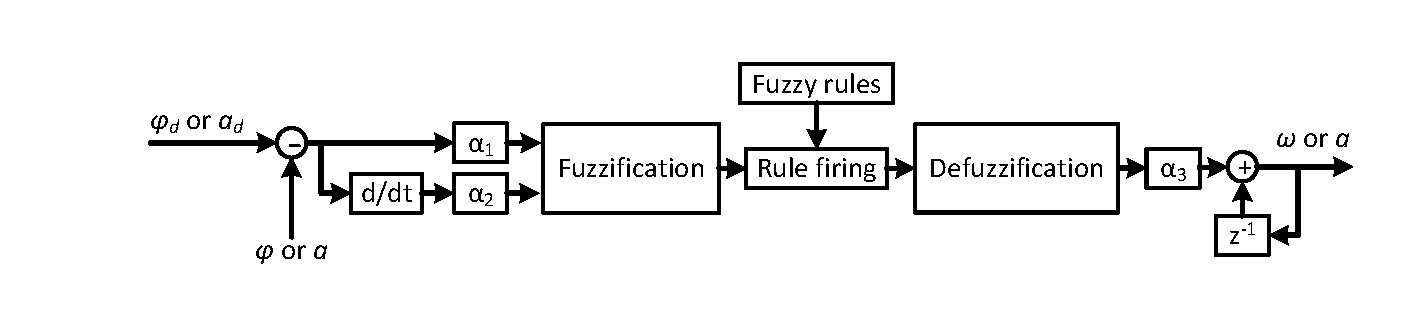
\includegraphics[width=0.9\linewidth]{Fuzzy_controller.pdf}
    \caption{Fuzzy controller used in phase ($\phi_d, \phi, \omega$) or displacement ($a, a_d$) tracking loops. $z^{-1}$ is the delay operator.}
    \label{F_fuzzy_diagram}
\end{figure*}


\begin{figure}
    \centering    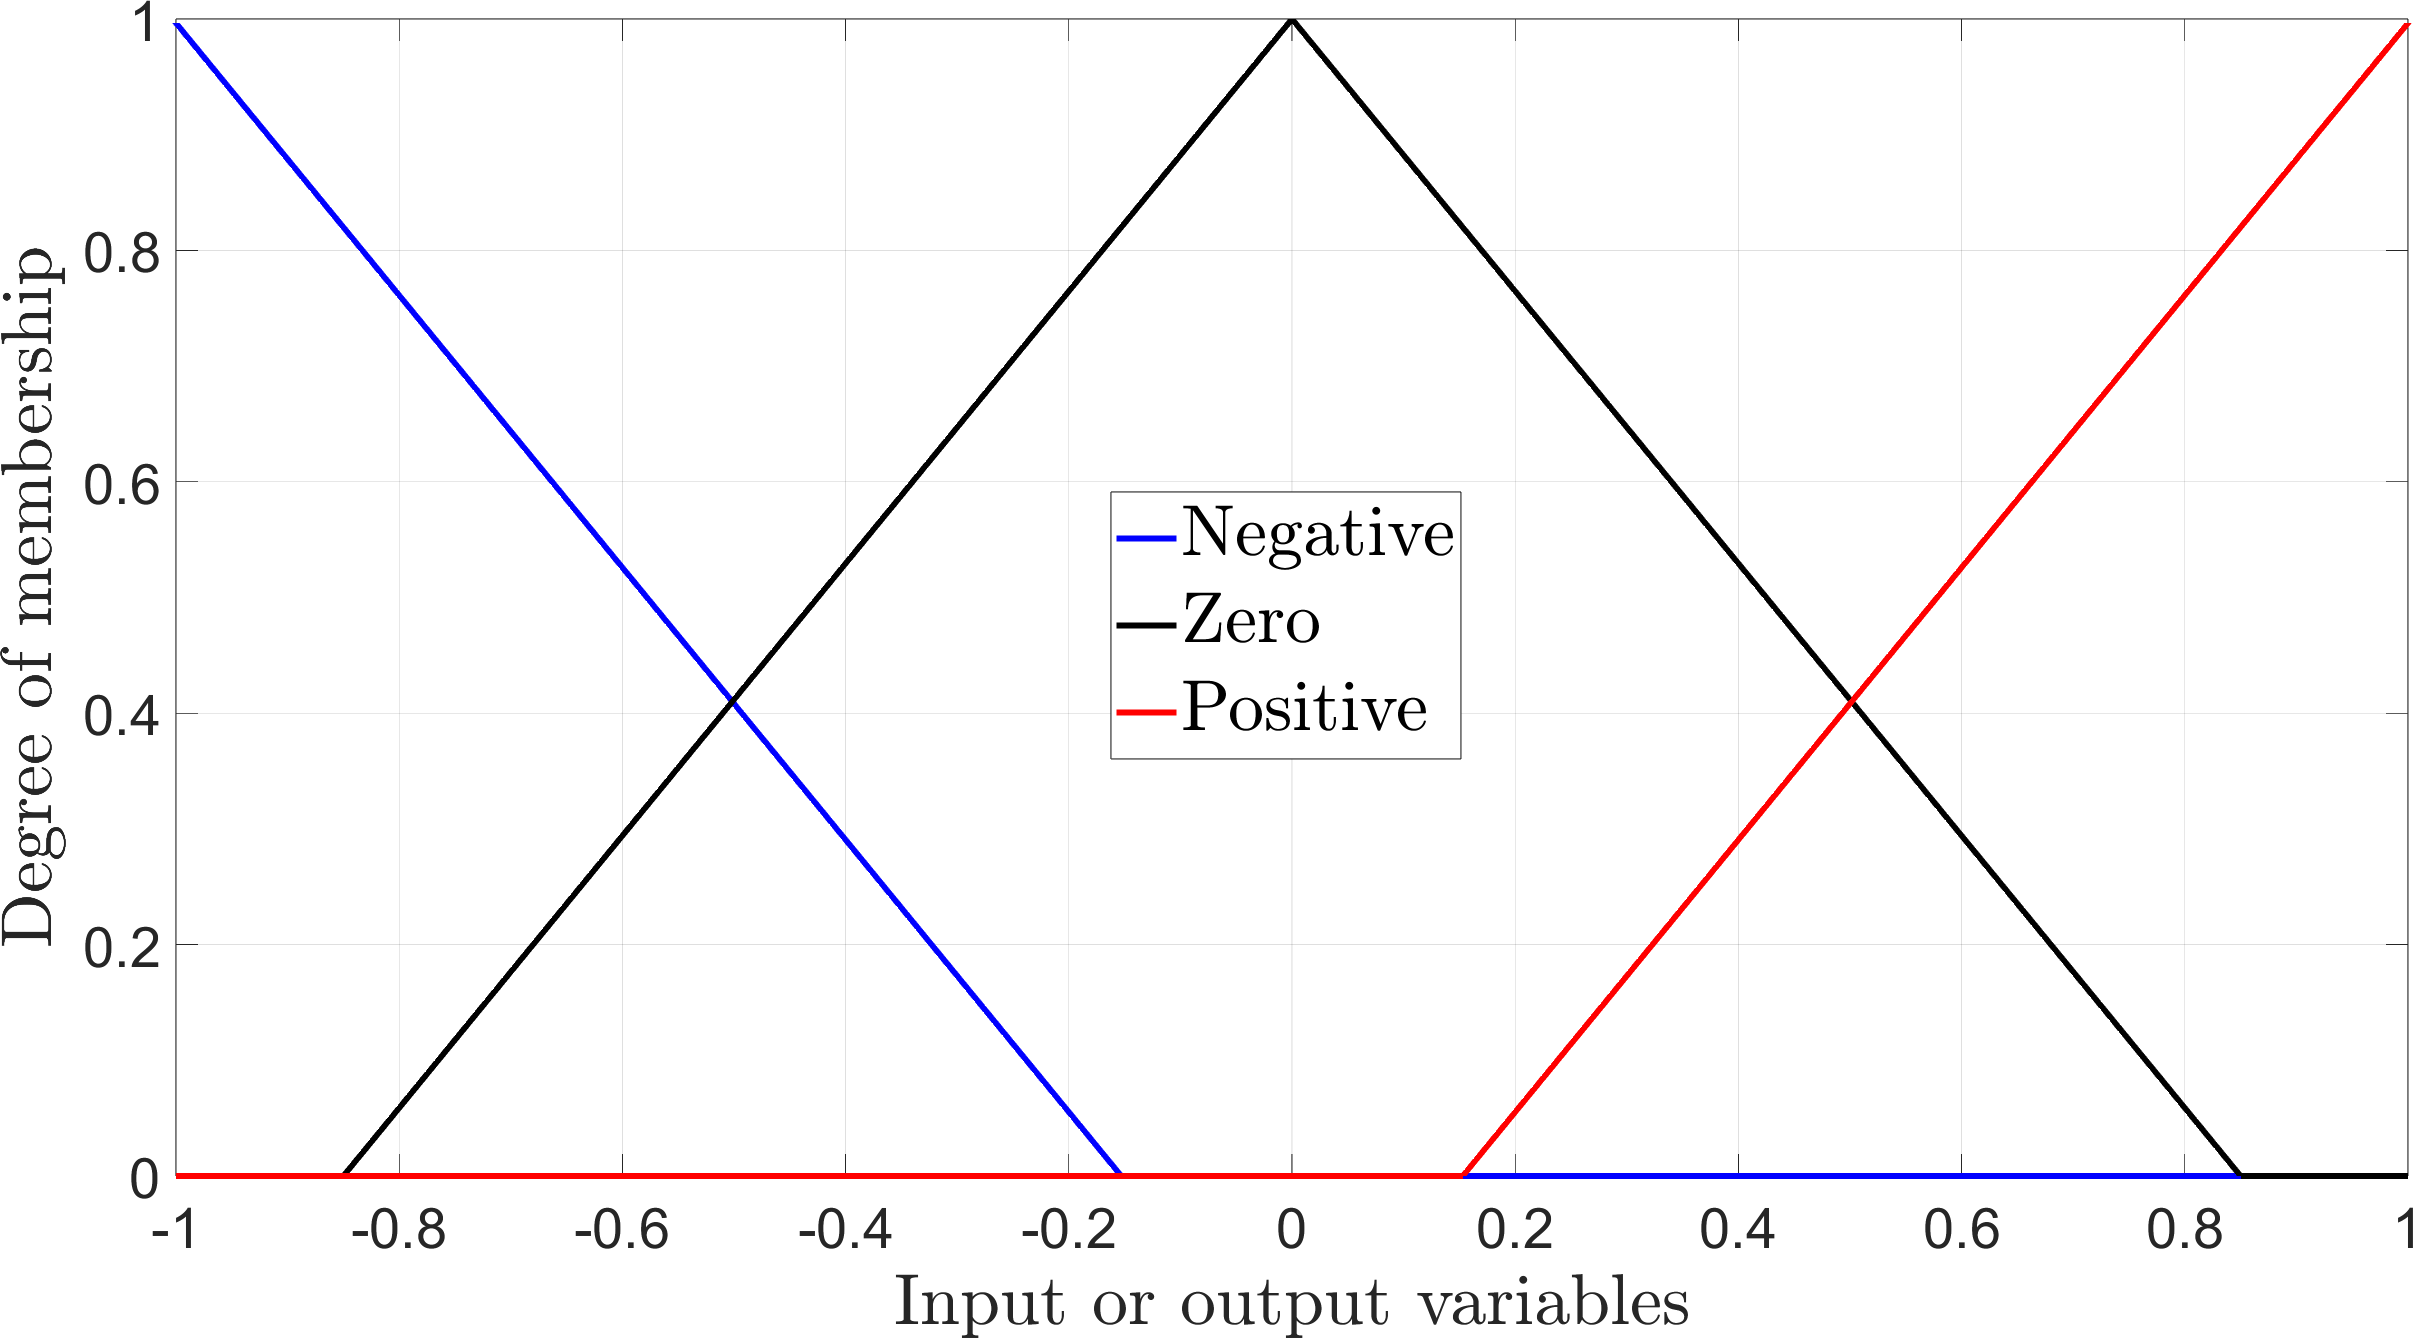
\includegraphics[width=\linewidth]{F_membership.png}
    \caption{Fuzzy memberships for both inputs and outputs, which are used for both phase and displacement tracking loops.}
    \label{F_fuzzy_memberships}
\end{figure}


\begin{figure}
    \centering    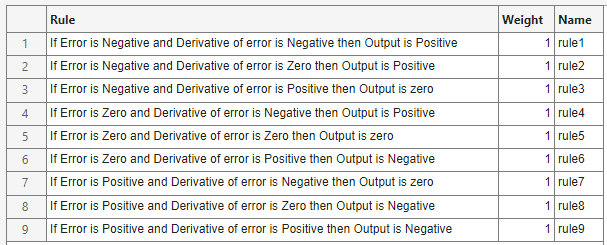
\includegraphics[width=\linewidth]{Fuzzy_rules.png}
    \caption{Fuzzy rules used for both phase and displacement tracking loops}
    \label{F_fuzzy_rules}
\end{figure}

The fuzzy controller illustrated in \Cref{F_fuzzy_diagram} is based on the Mamdani fuzzy inference system \cite{Ross2010}. It employs the same set of fuzzy rules for both the phase and displacement tracking loops, with each loop distinguished by its own scaling parameters ($\alpha_1, \alpha_2, \alpha_3$). The controller takes the error and its time derivative as inputs to compute the control signals. Notably, the same membership functions are applied to all input (error and its derivative) and output (control signal) variables, as shown in \Cref{F_fuzzy_memberships}.



\subsubsection{Phase detection} \label{S_phase_detection}

As it was seen in \Cref{S_frequency_seeking}, the phase between the input force $f$ and the output position $x_1$ must be detected to be used in the phase tracking controllers. \Cref{Lemma_phase_detection} can be used to detect such a phase.
\begin{theorem} \label{Lemma_phase_detection}
Assuming that the input force is $f(t)=a\sin(\omega t)$ the cosine angle between the input force $f$ and the output position $x_1$ in the steady-state can be calculated as follows:
\begin{equation}
\theta\triangleq \cos(\phi) = \frac{2} {a\gamma}\LF \{f(t)x_1(t) \} ,
\label{E_phase_calculated}
\end{equation}
where $\LF\{\cdot\}$ is a low-pass filter capable of cutting the angular frequency component $2\omega$, and $\gamma \in \mathbb{R}>0$.
\end{theorem}
\noindent \textbf{Proof.}
Applying the input force \Cref{E_F_resonance} to the system \Cref{E_plant_no_output} gives:
\begin{equation}
\ddot{x}_1(t)+\frac{k}{m}x_1(t)+\frac{b}{m} \dot{x}_1(t) =\frac{a}{m}\sin(\omega t) .
\label{E_plant_closed_loop}
\end{equation}
The dynamic response of \Cref{E_plant_closed_loop} reads as:
\begin{equation}
x_1(t)=x_{1h}+x_{1p},
\end{equation}
where $x_{1h}$ and $x_{1p}$ are the homogeneous and particular solutions. In the steady state, one has $x_{1h} \rightarrow 0$. Hence, for $x_{1h}=0$ and substituting the particular solution $x_{1p}$ one has 
\begin{equation}
x_1(t)=x_{1p}=\gamma\sin(\omega t+\phi).
\label{E_x_1_steady}
\end{equation}
Multiplying $f$ from \Cref{E_F_resonance} by $x_1$ from \Cref{E_x_1_steady} gives:
\begin{equation}
\begin{array}{l}
f(t)x_1(t)=a\gamma\sin(\omega t)\sin(\omega t+\phi)=\frac{a\gamma}{2}\cos(\phi)- \vspace{0.1cm} \\ 
\frac{a\gamma}{2}\cos(2\omega t +\phi) .
\end{array}
\label{E_multiple_avant}
\end{equation}
Hence, multiplication of the input force $f$ by the measured position $x_1$ gives a constant term$\frac{a\gamma}{2}\cos(\phi)$ plus a time-variable term $-\frac{a\gamma}{2}\cos(2\omega t +\phi)$. Hence, passing both sides through a low-pass filter to filter out the angular frequency component $2\omega$ one has:
\begin{equation}
\begin{array}{l}
\LF \{f(t)x_1(t) \}=\frac{a\gamma}{2}\cos(\phi)  \rightarrow  \phi =\cos^{-1} (\theta)= \vspace{0.1cm} \\ 
\cos^{-1} \big( \frac{2} {a\gamma}\LF \{f(t)x_1(t) \} \big) .
\end{array}
\label{E_multiple_avant_filter}
\end{equation}
 $\blacksquare$


 Calculating the phase using \Cref{E_multiple_avant_filter} may not be practical because the force $f$ may not be measured accurately. Alternatively, two position sensors can be employed to measured the phase, rather than using a force sensor, as explained in \Cref{R_practical_phase_detection}.
\begin{remark} \label{R_practical_phase_detection}
The cosine of the phase difference, {\em i.e.}, $\theta$ can be alternatively detected and served as the control variable in practice without measuring the force $f$ using an extra accelerometer sensor $a_0$ installed on the shaker as follows:
\begin{equation}
\theta\triangleq \cos(\phi) = -\frac{2} {\omega_d^2 m_0a\gamma}\LF \{a_0(t) x_1(t) \} ,
\label{E_phase_measured}
\end{equation}
where $m_0>0$ is the equivalent mass of the actuator and specimen, and $a_0$ is the shaker acceleration.
\end{remark} 
\noindent \textbf{Proof.}
From the Newton's second law one has $f(t)=m_0 a_0(t)$, where $a_0(t)$ is the acceleration of the actuator. Assuming that $f(t)=\sin(\omega_d t)$ is a pure sinusoidal function of time, one has $a_0(t)=(1/m_0)\sin(\omega_d t)$. Substituting this value into \Cref{E_multiple_avant_filter} gives \Cref{E_phase_measured}.
$\blacksquare$


\begin{table}
    \centering
    \begin{tabular}{|l|l|} \hline
     Ref.    &  Phase tracking controller  \\ \hline
    \cite{George_2006}  &  An unknown closed-loop controller \\  \hline
      \cite{Ji_2010}   &  Fuzzy controller  \\ \hline
    \cite{SCHRAMM2024117045,SCHNEIDER2018171,herrmann2018simulation_Thesis}  &  Constant frequency $\omega_d$ \\ \hline
    \cite{Su2014} & A commercial controller (Spectral Dynamics Puma) \\ \hline
    \cite{Dupke2026} & A commercial controller (LMS SCADAS) \\ \hline
    \cite{DORANGA2024115368} & PI controller \\
    \hline
    \end{tabular}
    \vspace{0.1cm}
    \caption{Phase tracking controllers developed for the resonance-based fatigue testing machines}
    \label{T_frequency_seeking}
\end{table}


\subsection{Displacement tracking} \label{S_amplitude_tracking}

In addition to the frequency/phase tracking discussed in \Cref{S_frequency_seeking}, the second objective is to control the specimen's displacement $x_1$ during testing to comply with standards such as DIN 50100 \cite{DIN_standard}. Substituting $s = j\omega$ into \Cref{E_Laplace} yields:
\begin{equation}
\frac{X_1}{F}=\frac{1}{-m\omega^2+bj\omega+k} .
\label{E_Laplace_frequency}
\end{equation}
The amplitude of \Cref{E_Laplace_frequency} reads as:
\begin{equation}
\big|\frac{X_1}{F}\big|=\frac{1}{\sqrt{(m\omega^2-k)^2+(b\omega)^2}}.
\label{E_Laplace_frequency_mag}
\end{equation}
For the resonance frequency $\omega=\omega_d$ calculated in \Cref{E_TF_standard_2}, the gain of the system \Cref{E_Laplace_frequency_mag}, during the resonance, is
\begin{equation}
|\frac{X_1}{F}|_{\omega=\omega_d}=\frac{m}{kb^2}.
\label{E_Laplace_frequency_mag_resonance}
\end{equation}
The homogeneous solution $x_{1h}$ of \Cref{E_plant_closed_loop} is zero in the steady state condition. In this case, for \Cref{E_F_resonance}, and according to \Cref{E_x_1_steady}, $x_1$ presents a sinusoidal response in the resonance as follows:
\begin{equation}
x_1(t)=a_0 \frac{m}{kb^2} \sin(\omega_d t+\pi/2).
\label{E_x_1_steady_amplitude}
\end{equation}
Assuming that $a_d$ is the desired amplitude of $x_1$, the amplitude of the input force can be calculated as follows.
\begin{equation}
\begin{array}{l}
x_1(t)=a_0 \frac{m}{kb^2} \sin(\omega_d t+\pi/2) = a_d  \sin(\omega_d t+\pi/2) \rightarrow \vspace{0.1cm} \\ 
a_0=a_d \frac{kb^2}{m}. 
\end{array}
\label{E_x_1_steady_a0}
\end{equation}
It leads to the following open-loop force:
\begin{equation}
F(t)=a_d \frac{kb^2}{m} \sin(\omega_dt). 
\label{E_x_1_open_loop_force}
\end{equation}
Similar to the discussion in \Cref{S_frequency_controller} regarding phase tracking, calculating the excitation force based on \Cref{E_x_1_open_loop_force} may not guarantee the required performance—such as maintaining the specimen's displacement within 3\% of the desired value $a_d$, as specified in the DIN 50100 standard \cite{DIN_standard}—due to the uncertain and time-varying nature of the parameters $k$, $b$, and $m$ during testing. Therefore, the force amplitude $a_0$ must be adjusted using a closed-loop control law. The only closed-loop controller explained in the literature for this purpose is the PI controller, which may be used in conjunction with a time-clocked state machine algorithm to synchronize the imbalance motors \cite{SCHRAMM2024117045,SCHNEIDER2018171,herrmann2018simulation_Thesis}. In this configuration, $a_0$ becomes time-varying and is computed as follows:
\begin{equation}
\begin{array}{l}
u_2(t) \triangleq x_0(t)=k_{p} (\max_{T_d}(x_1(t))-a_d) + \vspace{0.1cm} \\
k_{i} \int (\max_{T_d}(x_1(t))-a_d) dt + k_d \dot{x}_1(t),
\end{array}
\label{E_PID_amplitude}
\end{equation}
where, $u_2(t)$ denotes the closed-loop control signal used to adjust the excitation force amplitude. The constants $k_p$, $k_i$, and $k_d$ are the proportional, integral, and derivative gains, respectively—equivalent to those defined in \Cref{E_frequency_PID}. The term $T_d = 1/\omega_d$ represents the period corresponding to the resonance frequency, and $\max\limits_{T_d}(\cdot)$ denotes the maximum value over one period $T_d$. As with the PID controller in \Cref{E_frequency_PID} used for phase tracking, the tuning of parameters for this closed-loop controller has not been addressed in the literature. Consequently, the selection of appropriate values for $k_p$, $k_i$, and $k_d$ to ensure both stability and performance remains unclear (see also the phase-tracking PI controller design for piezoelectric systems in \cite{s22176378}).

\subsection{Instrumentation} \label{S_instrumentation}

To implement the phase and amplitude tracking control algorithms discussed in \Cref{S_frequency_seeking,S_amplitude_tracking}, various sets of instrumentation are employed in the literature, including sensors, actuators, and computing platforms. An overview of these instrumentation configurations is provided in \Cref{T_machine_types}. Additionally, an insightful historical review of the computers used in vibration test controllers can be found in \cite{Computers}.







\begin{sidewaystable}
    \centering
    \begin{tabular}{|l|l|l|l|c|c|} \hline
     Ref.   &  Actuator  & Sensor & Computer &  Freq. &  Acc. \\ \hline
     \cite{SCHRAMM2024117045}   & Imbalance motors &   Strain gauge, laser sensor and force transducer & FPGA  & 14Hz &    $\pm 4\%$\\ \hline
\cite{SCHNEIDER2018171}   & Imbalance motors elements  &  Strain gauge, laser sensor and force transducer & FPGA  & 20Hz  &   N/A \\  \hline

\cite{herrmann2018simulation_Thesis} & Imbalance motors &   Strain gauge, laser sensor and force transducer  & FPGA   & 80Hz &  $\pm 1.98\%$  \\    \hline

\cite{feng2003development_Japaneese}   & Electrodynamic shaker &  Dynameter for force measurement  & 80c196 microcontroller & 100Hz  &  $\pm 1.5\%$ \\ \hline

\cite{Su2014} & Electrodynamic shaker   & N/A & N/A &  523Hz & N/A   \\ \hline

\cite{George_2006} & Electrodynamic shaker    & CEA-05-062UW-350 strain gages & N/A  &  1600Hz & N/A \\ \hline
\cite{CESNIK20125370} & LDS V555 shaker  &  Accelerometer & CompactRIO &  794Hz &  N/A \\  \hline
\cite{gautrelet2020resonance} & Electrodynamic shaker &  Strain gauge, accelerometer,  crack gauge &  N/A & 320Hz & N/A  \\  \hline 


\cite{Ji_2010} &  PLG-100 Electro-hydraulic & N/A & N/A  &  N/A  & N/A  \\  \hline


\cite{DORANGA2024115368} & Electrodynamic shaker & Laser sensor & N/A  & 178Hz & N/A \\ \hline

\cite{Rouillard_2000} & Electro-hydraulic shaker & N/A & PC & 14.5Hz & N/A \\\hline

\cite{Stanzl01041980_fast_ultrasonic} & Ultrasonic transducer & Magnetic coil  & N/A  & 20kHz & N/A \\
           \hline
    \end{tabular}
    \vspace{0.1cm}
    \caption{Different structures of resonance-based fatigue testing machines. Freq. stands for the maximum resonance frequency used in the experiments. Acc. stands for the worst amplitude accuracy.}
    \label{T_machine_types}
\end{sidewaystable}



\section{The proposed method: sliding-mode control system} \label{S_SMC}

This section aims to develop a more reliable control system for resonance-based fatigue testing machines using the twisting sliding-mode control algorithm, addressing the limitations of previously reviewed control strategies—such as lack of robustness, absence of formal stability guarantees, and insufficient performance. By applying a pure sinusoidal input force of the form $F = u_2 \sin(u_1 t)$ to \Cref{E_plant_no_output}, one obtains:
\begin{subequations}
  \begin{empheq}[left=\empheqlbrace]{align}
\dot{x}_1(t)&=x_2(t) \label{E_plant_no_output_with_control_input_1} \\
\dot{x}_2(t)&=-\frac{k}{m} x_1(t) -\frac{b}{m} x_2(t) + \frac{u_2}{m} \sin(u_1 t) , \label{E_plant_no_output_with_control_input_2} 
  \end{empheq}
\label{E_plant_no_output_with_control_input}
\end{subequations}
where $u_1 = \omega$ (the frequency of the excitation force) and $u_2(t) = a$ (the amplitude of the excitation force) are the closed-loop control signals. These two control input signals are designed based on the twisting sliding-mode algorithm in this section to achieve two objectives, {\em i.e.}, tracking the desired phase $\phi_d$ and displacement $a_d$. This is equivalent to tracking the following sinusoidal trajectory by $x_1$:
\begin{equation}
x_1(t) \rightarrow x_{1d}(t)=a_d\sin(\omega_d t+\phi_d) .
\label{E_obj}
\end{equation}
Equations \Cref{E_plant_no_output_with_control_input} describe a time-varying, nonlinear, and multivariable system that does not follow any conventional control-oriented form, making it unclear how to design the two control inputs $u_1(t)$ and $u_2(t)$ to achieve the objective in \Cref{E_obj}. To address this challenge, an alternative control-oriented model is developed in \Cref{S_identification}, based on identification methods applied to \Cref{E_plant_no_output_with_control_input}, to facilitate controller design. This model is derived from offline numerical simulations leading to several sources of uncertainties because of the potential different behavior of the model \Cref{E_plant_no_output_with_control_input} and real system. Hence, a robust control strategy is required to manage uncertainties such as unmodeled dynamics. To this end, a sliding-mode control law is developed for the identified system in \Cref{S_SMC_design}, ensuring robust closed-loop stability.

\subsection{Control-oriented model} \label{S_identification}


Two mathematical models are identified to describe the resonance and amplitude dynamics as explained in \Cref{S_frequency_model,S_amplitude_model}, respectively. 



\subsubsection{Frequency to phase model ($u_1=\omega \rightarrow z_2=\theta$)} \label{S_frequency_model}


The first mathematical model establishes a dynamic relationship between the frequency $\omega$ and the cosine of the phase angle, {\em i.e.}, $\theta = \cos(\phi)$. The general form of the identified models is given as follows:
\begin{subequations}
  \begin{empheq}[left=\empheqlbrace]{align}
\dot{z}_1(t)&=z_2(t) \label{E_plant_identified_model_1} \\
\dot{z}_2(t)&=pz_2+qu_1(t) , \label{E_plant_identified_model_2} 
  \end{empheq}
\label{E_plant_identified_model}
\end{subequations}
where $u_1 = \omega$ is the control input, $z_1 = \int \theta , dt$ and $z_2 = \theta$ are the state variables, and $p \in \mathbb{R}$ and $q \in \mathbb{R}$ are two functions to be estimated. To this end, the {\fontfamily{qcr}\selectfont System Identification Toolbox} in {\fontfamily{qcr}\selectfont MATLAB} is employed in this work on the system \Cref{E_plant_no_output}, with parameters $m = 0.01772$~kg, $k = 256$~N/m, and $b = 0.12$~Ns/m (these parameters are selected based on experimental tests to ensure that \Cref{E_plant_no_output} accurately reflects the behavior of the real specimen). The frequency $u_1 = \omega$ is varied stepwise around the resonance frequency $\omega_d = 39$~rad/s, and the identified functions $p$ and $q$ are listed in \Cref{T_identification}. As observed, the system parameters vary depending on the operating pint $\omega$. This issue is addressed in \Cref{S_SMC_design} through a robust controller design. Assuming that $p$ and $q$ consist of known components ($\bar{p}$ and $\bar{q}$) and unknown or uncertain parts ($\tilde{p}$ and $\tilde{q}$), one has:

\begin{subequations}
  \begin{empheq}[left=\empheqlbrace]{align}
p=\bar{p}+\tilde{p} \label{E_p} \\
q=\bar{q}+\tilde{q} . \label{E_qq} 
  \end{empheq}
\label{E_p_q}
\end{subequations}


\begin{table}
    \centering 
    \begin{tabular}{|l|c|c|} \hline
       $\omega (\rad/s)$   & $p$ & $q$  \\ \hline
  $5 \rightarrow 6$   & $-1.424$ & $50.16 \times 10^{-5} $  \\ \hline 
  $20 \rightarrow 21$   & $-1.093$ & $10.7 \times 10^{-5} $  \\ \hline 
  $38 \rightarrow 39$   & $-1.041$ & $5.88 \times 10^{-5} $  \\ \hline 
    \end{tabular}
    \vspace{0.1cm}
    \caption{Identification of $p$ and $q$ around different $\omega$ for the system \Cref{E_plant_no_output_with_control_input} with $m=0.01772$~kg, $k=256$~N/m, and $b=0.12$~Ns/m}
    \label{T_identification}
\end{table}









\subsubsection{Force amplitude to resonance amplitude model ($u_2=a \rightarrow z_2=\max\limits_{T_d}(x_1(t))$)} \label{S_amplitude_model}
The other model describes the mathematical relationship between the force amplitude $u_2 = a$ and the resonance amplitude error over a period, {\em i.e.}, $e_2 = \max\limits_{T_d}(x_1(t)) - a_d$, $e_1 = \int (\max\limits_{T_d}(x_1(t)) - a_d) , dt$. Similar to the identification method introduced in \Cref{S_frequency_model}, the functions $p$ and $q$ are approximated as listed in \Cref{T_identification_amplitude}. Note that the general form of the model in this case reads as:
\begin{subequations}
  \begin{empheq}[left=\empheqlbrace]{align}
\dot{e}_1(t)&=e_2(t) \label{E_plant_identified_model_e_1} \\
\dot{e}_2(t)&=pe_2+pa_d+qu_2(t) . \label{E_plant_identified_model_e_2} 
  \end{empheq}
\label{E_plant_identified_model_e}
\end{subequations}
The proposed amplitude controller will be designed in \Cref{S_SMC_design} to handle such unmodeled dynamics. 





\begin{table}
    \centering 
    \begin{tabular}{|l|c|c|} \hline
       $\omega (\rad/s)$   & $p$ & $q$  \\ \hline
       5   & $-8.259$ & $0.008093$  \\ \hline
         20   & $-34.7$ & $0.03425$  \\ \hline
       38   & $-68.08$ & $0.06748$  \\ \hline
    \end{tabular}
    \vspace{0.1cm}
    \caption{Identification of $p$ and $q$ for \Cref{E_plant_identified_model_e} when the amplitude of the input force $a$ changes stepwise from 0 to 1 for the indicated frequencies with $m=0.01772$~kg, $k=256$~N/m, and $b=0.12$~Ns/m}
    \label{T_identification_amplitude}
\end{table}


\subsection{Twisting controller design} \label{S_SMC_design}

This section aims to design the control signals $u_1$ and $u_2$. Various control algorithms can be applied to the control-oriented models \Cref{E_plant_identified_model,E_plant_identified_model_e}. In this study, the twisting algorithm is adopted for the sliding-mode controller design to address the unmodeled dynamics and parameter uncertainties present in the identified model \Cref{E_p_q}, while also ensuring finite-time convergence in theory. The SMC design for phase and displacement tracking is discussed in \Cref{S_SMC_phase} and \Cref{S_SMC_amplitude}, respectively.

\subsubsection{TC for the phase tracking} \label{S_SMC_phase}

To keep the system on the resonance frequency, the phase $\phi$ must converge to $\pi/2$ for $\zeta \approx 0$, or alternatively $\phi=\cos(\theta) \rightarrow 0$. The twisting controller is proposed as follows to achieve this objective:
\begin{equation}
u_1(t) =  -\frac{\bar{p}}{\bar{q}}z_2 -b_1 \sgn(z_1) -b_2 \sgn(z_2),
\label{E_TC}
\end{equation}
where $b_1$ and $b_2$ are the TC gains, and $\sgn(\cdot)$ is the signum function defined below:
\begin{equation}
\sgnsingle(s) \triangleq \left \{
    \begin{array}{lcl}
  -1   & \for & s\in \mathbb{R}^- \\
0  & \for & s=  0 \\
   +1  & \for & s \in \mathbb{R}^+  . \\
    \end{array}
    \right.
    \label{E_sgn_function}
\end{equation}
  Substituting \Cref{E_TC,E_p_q} into \Cref{E_plant_identified_model} the following closed-loop equation is obtained:
\begin{subequations}
  \begin{empheq}[left=\empheqlbrace]{align}
\dot{z}_1(t)&=z_2(t) \label{E_plant_closed_loop_phase_1} \\
\dot{z}_2(t)& = (p-\bar{p}\frac{q}{\bar{q}})z_2-q(b_1 \sgn(z_1) + \notag \\
& b_2 \sgn(z_2)) . \label{E_plant_closed_loop_phase_2} 
  \end{empheq}
\label{E_plant_closed_loop_phase}
\end{subequations}



\begin{theorem}[\cite{Levant_TC,Levant_TC_geometry,Orlov_twisting,Oza_twisting,POLYAKOV_twisting,Santiesteban_twisting}] \label{Theorem_TC_phase}
Assuming that $p$ and $q$ satisfy the conditions $|(p-\bar{p}\frac{q}{\bar{q}})z_2|\leq k_a$ and $0\leq k_m  \leq |q| \leq k_M$, and the parameters $b_1$ and $b_2$ satisfy the conditions
\begin{subequations}
  \begin{empheq}[left=\empheqlbrace]{align}
&(b_1+b_2)k_m-k_a> (b_1-b_2)k_M+k_a \label{E_cond_TC_1} \\
&(b_1-b_2)k_m>k_a, \label{E_cond_TC_2} 
  \end{empheq}
\label{E_cond_TC}
\end{subequations}
the closed-loop system \Cref{E_plant_closed_loop_phase} converges to the origin in finite-time.
\end{theorem}



\subsubsection{TC for the amplitude tracking} \label{S_SMC_amplitude}

In addition to the phase tracking controller addressed in \Cref{S_SMC_phase}, an amplitude tracking controller is designed in this section such that the resonance amplitude $\max\limits_{T_d}(x_1(t))$ tracks the desired one $a_d$. To this end, the model \Cref{E_plant_identified_model_e} is considers in this section. The design procedure is similar to the one presented in \Cref{S_SMC_phase}, and for the sake of space, only the final results are presented. The continuous-time amplitude tracking twisting controller is:
\begin{equation}
u_2(t) =  -\frac{\bar{p}}{\bar{q}}(e_2+a_d) -b_1 \sgn(e_1) -b_2 \sgn(e_2).
\label{E_TC_amplitude}
\end{equation}
Substituting \Cref{E_TC_amplitude} into \Cref{E_plant_identified_model_e} gives:
\begin{subequations}
  \begin{empheq}[left=\empheqlbrace]{align}
\dot{e}_1(t)&=e_2(t) \label{E_plant_closed_loop_a_plitude_1} \\
\dot{e}_2(t)& = (p-\bar{p}\frac{q}{\bar{q}})(e_2+a_d)-q(b_1 \sgn(e_1) + \notag\\
& b_2 \sgn(e_2)) , \label{E_plant_closed_loop_plitude_2} 
  \end{empheq}
\label{E_plant_closed_loop_plitude}
\end{subequations}
In this case, \Cref{Theorem_TC_phase} leads to:
\begin{corollary}[\cite{Levant_TC,Levant_TC_geometry,Orlov_twisting,Oza_twisting,POLYAKOV_twisting,Santiesteban_twisting}] \label{Theorem_TC_amplitude}
Assuming that $p$ and $q$ satisfy the conditions $|(p-\bar{p}\frac{q}{\bar{q}})(e_2+a_d)|\leq k_a$ and $0\leq k_m  \leq |q| \leq k_M$, and the parameters $b_1$ and $b_2$ satisfy the conditions
\begin{subequations}
  \begin{empheq}[left=\empheqlbrace]{align}
&(b_1+b_2)k_m-k_a> (b_1-b_2)k_M+k_a \label{E_cond_TC_amplitude_1} \\
&(b_1-b_2)k_m>k_a, \label{E_cond_TC_amplitude_2} 
  \end{empheq}
\label{E_cond_TC_amplitude}
\end{subequations}
the closed-loop system \Cref{E_plant_closed_loop_plitude} converges to the origin in finite-time.
\end{corollary}

\begin{remark} \label{R_chattering}
    The control laws \Cref{E_TC,E_TC_amplitude} are expressed in the continuous-time domain, which cannot be directly implemented on the digital computers used for the numerical simulations and experiments. Hence, a time-discretization must be used to obtain a digital version of \Cref{E_TC}. Following the literature, the Euler forward discretization of \Cref{E_TC} leads to the numerical chattering, {\em i.e.}, high-frequency oscillations on the control signals $u_1$ and $u_2$ causing performance deterioration, excitation of unmodeled dynamics, actuator degradation, and even instability. Hence, the deadbeat implementation technique \cite{MOJALLIZADEH_Franklin} is used in this study to avoid the chattering while keeping the properties of the continuous-time TC \Cref{E_TC}, such as the finite-time convergence, after the discretization. This implementation is detailed in \Cref{S_appendix}.
\end{remark}


\section{Numerical simulations} \label{S_simulations}

The block diagram of the implemented control systems is shown in \Cref{F_control_diagram}. The {\fontfamily{qcr}\selectfont Phase detection} block, described in \Cref{E_multiple_avant_filter}, is used to calculate the phase. This value is then fed into the {\fontfamily{qcr}\selectfont frequency controller}. Meanwhile, the displacements are calculated using $\max\limits_{T_d}(x_1(t))$ and are provided to the {\fontfamily{qcr}\selectfont displacement controller}. As previously explained, the system requires two control laws—namely, the frequency and amplitude controllers—to synthesize the control signals $u_1$ and $u_2$, thereby achieving phase and displacement tracking, respectively. These two controllers are implemented using three different methods: twisting, PI, and fuzzy algorithms, as detailed in \Cref{S_designed_TC,S_designed_PI,S_designed_fuzzy}, respectively.



\begin{figure*}
    \centering    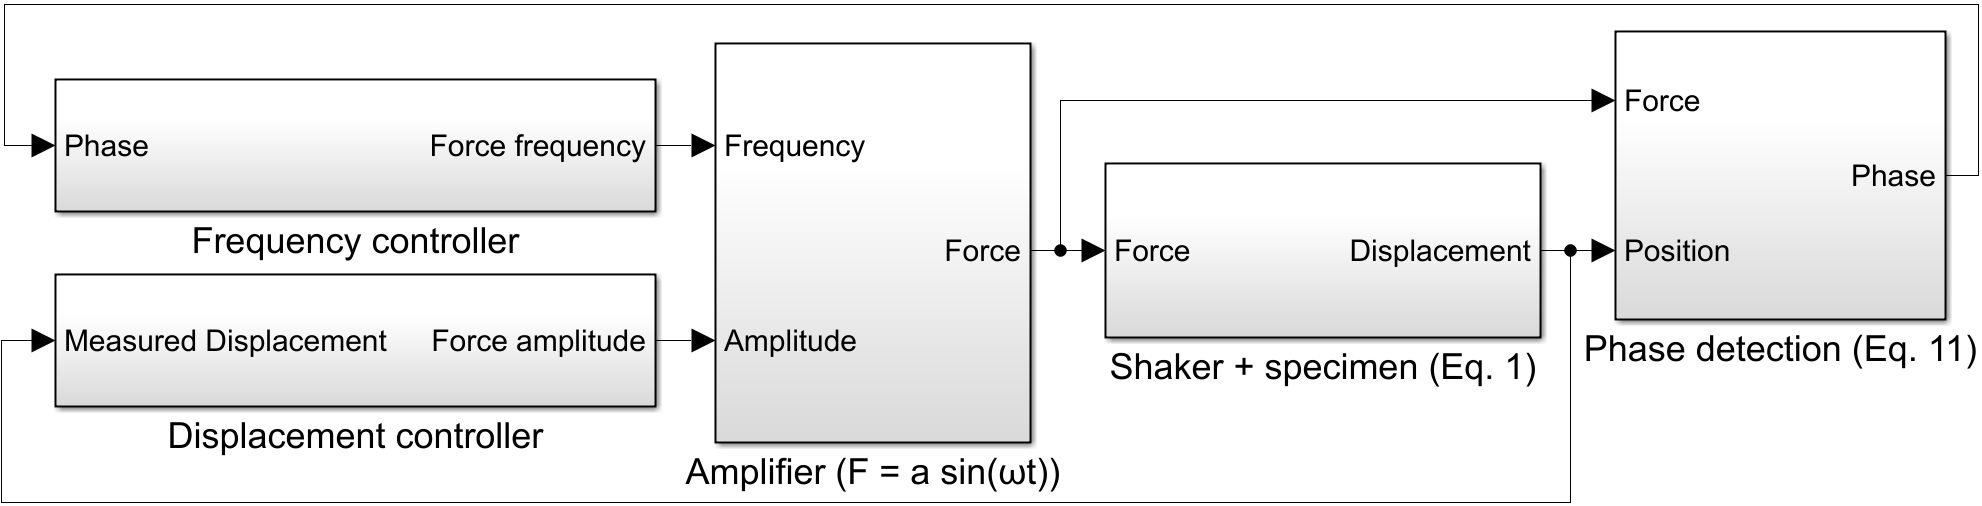
\includegraphics[width=\linewidth]{F_simulink.png}
    \caption{Block diagram of the implemented control system in {\fontfamily{qcr}\selectfont Simulink} }
    \label{F_diagram}
\end{figure*}




\subsection{The twisting controller} \label{S_designed_TC}

The developed twisting control signals $u_1$ and $u_2$ in the continuous-time setting are shown in \Cref{E_TC,E_TC_amplitude}, respectively. However, these control signals contain the signum function, which is sensitive to time discretization \cite{MOJALLIZADEH_Franklin}. Due to the small sampling time used in the numerical simulations, the TC is implemented explicitly (see \Cref{E_TC_a2_explicit}) without exhibiting chattering. However, as will be seen in \Cref{S_experiments}, the large sampling time of one second used in the practical experiments necessitates implementing the TC based on the deadbeat method which is detailed in the appendix in \Cref{S_appendix}. The parameters of the TC $b_1$ and $b_2$ can be calculated based on \Cref{Theorem_TC_amplitude,Theorem_TC_phase} and using the identified parameters listed in \Cref{T_identification,T_identification_amplitude}.

\subsection{PID controller} \label{S_designed_PI}

Following the literature, the PID controller has been widely employed in nearly all references where closed-loop phase tracking is required. However, its application to amplitude tracking has not yet been explored. The phase and amplitude tracking PID controllers described in \Cref{E_frequency_PID,E_PID_amplitude} require three parameters: $k_p$, $k_i$, and $k_d$. Nevertheless, the selection of these parameters to ensure control objectives such as stability remains unaddressed in the existing literature.

\begin{table}
    \centering
    \begin{tabular}{|l|c|c|} \hline 
\cellcolor{gray}  & Phase tracking loop  & Displacement tracking loop \\ \hline
PID & $k_p=43$,  $k_i=3$, $k_d=34$  & $k_p=229$,  $k_i=0.2$, $k_d=44$ \\ \hline
TC & $b_1=31$,  $b_2=77$  & $b_1=0.04$,  $b_2=0.1$ \\ \hline
Fuzzy & $\alpha_{1,2,3}=25, 5, 20$  & $\alpha_{1,2,3}=0.3, 0.1, 0.4$  \\  \hline
    \end{tabular}
    \vspace{0.1cm}
    \caption{Controllers' parameters tuned based on the objective function \Cref{E_objective}}
    \label{T_parameters}
\end{table}


\subsection{Fuzzy controller} \label{S_designed_fuzzy}

The same fuzzy controllers, with different scaling parameters $\alpha_1$, $\alpha_2$, and $\alpha_3$, are employed in the phase and displacement tracking loops. Details of the fuzzy controller are provided in \Cref{S_designed_fuzzy}. This controller receives the error and its time derivative, and computes the control signals according to \Cref{F_fuzzy_diagram}. For the phase tracking loop, the input variables are the phase $\phi$ and its time derivative $\dot{\phi}$, while the output is the frequency $\omega$. In contrast, for the displacement tracking loop, the inputs are the measured displacement $\max_{T_d}(x_1(t))$ and its time derivative, and the output is the amplitude of the excitation sinusoidal force $a$. Each fuzzy controller uses three scaling parameters, which are tuned using the unified optimization method described in \Cref{S_tuning}.


\subsection{Parameter tuning} \label{S_tuning}

As it was seen, each control architecture shares different parameters that must be tuned to provide fair comparisons among all the control methods. To this end, the parameters of all the mentioned controllers have been tuned based on the numerical simulations, where the objective is to minimize the following cost function.
\begin{equation}
\begin{array}{l}
J_x=\int (\max_{T_d}(x_1(t))-a_d)^2 \hspace{0.2cm}  dt \vspace{0.1cm} \\
J_\phi=\int  (\phi(t)-\phi_d)^2  \hspace{0.2cm}  dt \vspace{0.1cm}  \\
J=J_x+J_\phi ,
\end{array}
\label{E_objective}
\end{equation}
where $J_x$ and $J_\phi$ represent the displacement and phase tracking performances, respectively. As previously explained, $(\phi(t) - \phi_d)$ denotes the phase tracking error, while $\max_{T_d}(x_1(t)) - a_d$ corresponds to the displacement tracking error. The {\fontfamily{qcr}\selectfont particle swarm optimization} functions provided by {\fontfamily{qcr}\selectfont MATLAB} are employed for parameter tuning. The optimized parameters are summarized in \Cref{T_parameters}. It should be noted that special attention is paid to the parameter selection to avoid any significant displacement overshoots. Such overshoots are critical in fatigue testing, as they can lead to damage and render the fatigue testing machine non-compliant with standards and regulations.




\begin{table}
    \centering
    \begin{tabular}{|l|c|c|c|} \hline
       \cellcolor{gray}  &  TC  & PI & fuzzy   \\  \hline 
      $J_x$ & 0.0266  & 0.0387  &  0.0267   \\  \hline 
      $J_\phi$  & 0.0160  & 0.0259  & 0.0181    \\ \hline 
       $J$ &  0.0426 & 0.0646  &   0.0448 \\ \hline 
    \end{tabular}
    \vspace{0.1cm}
    \caption{Simulation: displacement and phase tracking performances}
    \label{T_J_simulation}
\end{table}



\section{Simulation results}

The numerical simulations are performed using the parameters listed in \Cref{T_parameters}, and the corresponding results are presented in \Cref{F_sim_frequency,F_sim_displacement}. The simulation runs for 180 seconds, with an abrupt reduction in the stiffness parameter $k$ from 256 N/m to 236 N/m at 120 seconds to simulate the appearance of a crack, thereby replicating realistic test conditions. This change is intended to evaluate the controllers' robustness in tracking both phase and displacement. The objective is to track the desired phase $\phi_d = 90^\circ$ to minimize energy consumption by operating at the peak amplitude of the Bode diagram, as shown in \Cref{F_Bode}. Note that the variable step size {\fontfamily{qcr}\selectfont ode45} solver is used for the numerical simulation, with a maximum sampling time of one millisecond to reduce discretization effects. In this case, the TC is implemented using the explicit discretization \Cref{E_TC_a2_explicit}, without showing any chattering.
According to \Cref{F_sim_frequency}, all controllers can achieve the desired $\phi_d = 90^\circ$ even in the presence of the perturbation at $t = 120$~s. Among the controllers, the TC achieves the desired phase slightly faster than the other two controllers, and its phase tracking is less affected by the perturbation at $t = 120$~s. Comparing the transient responses, the PID controller appears to exhibit the largest overshoots and the slowest convergence rate.
The other control objective is to track a displacement of 1.5~mm, as illustrated in \Cref{F_sim_displacement}. This value is determined by specialists in the fatigue analysis community for the selected specimen made of carbon fiber composite materials (see \Cref{F_setup}). The system under study is multivariable, meaning that the frequency and displacement control channels influence each other. Additionally, as shown in \Cref{F_Bode}, the amplitude changes significantly around the resonance frequency $\omega_d$. As a result, large oscillations are observed in \Cref{F_sim_displacement}, particularly during the transient phase. According to the results, all control methods achieve the desired displacement of 1.5~mm in the steady state. However, the TC and fuzzy methods show better responses than the PID. In addition, these two controllers demonstrate better disturbance rejection compared to the PID controller. Note that, as detailed in \Cref{S_tuning}, special attention is paid to parameter tuning to avoid any displacement overshoot that could cause early damage to the specimen and result in noncompliance with testing standards. As a result, no significant displacement overshoot is observed in \Cref{F_sim_displacement}. The quantified results corresponding to the simulations are presented in \Cref{T_J_simulation}, indicating that the TC and fuzzy controllers exhibit smaller tracking errors in both phase and displacement compared to the PID controller. This is likely due to the nonlinear dynamics present in the system, which cannot be effectively handled by a linear control law such as the PID.

\begin{figure}
    \centering    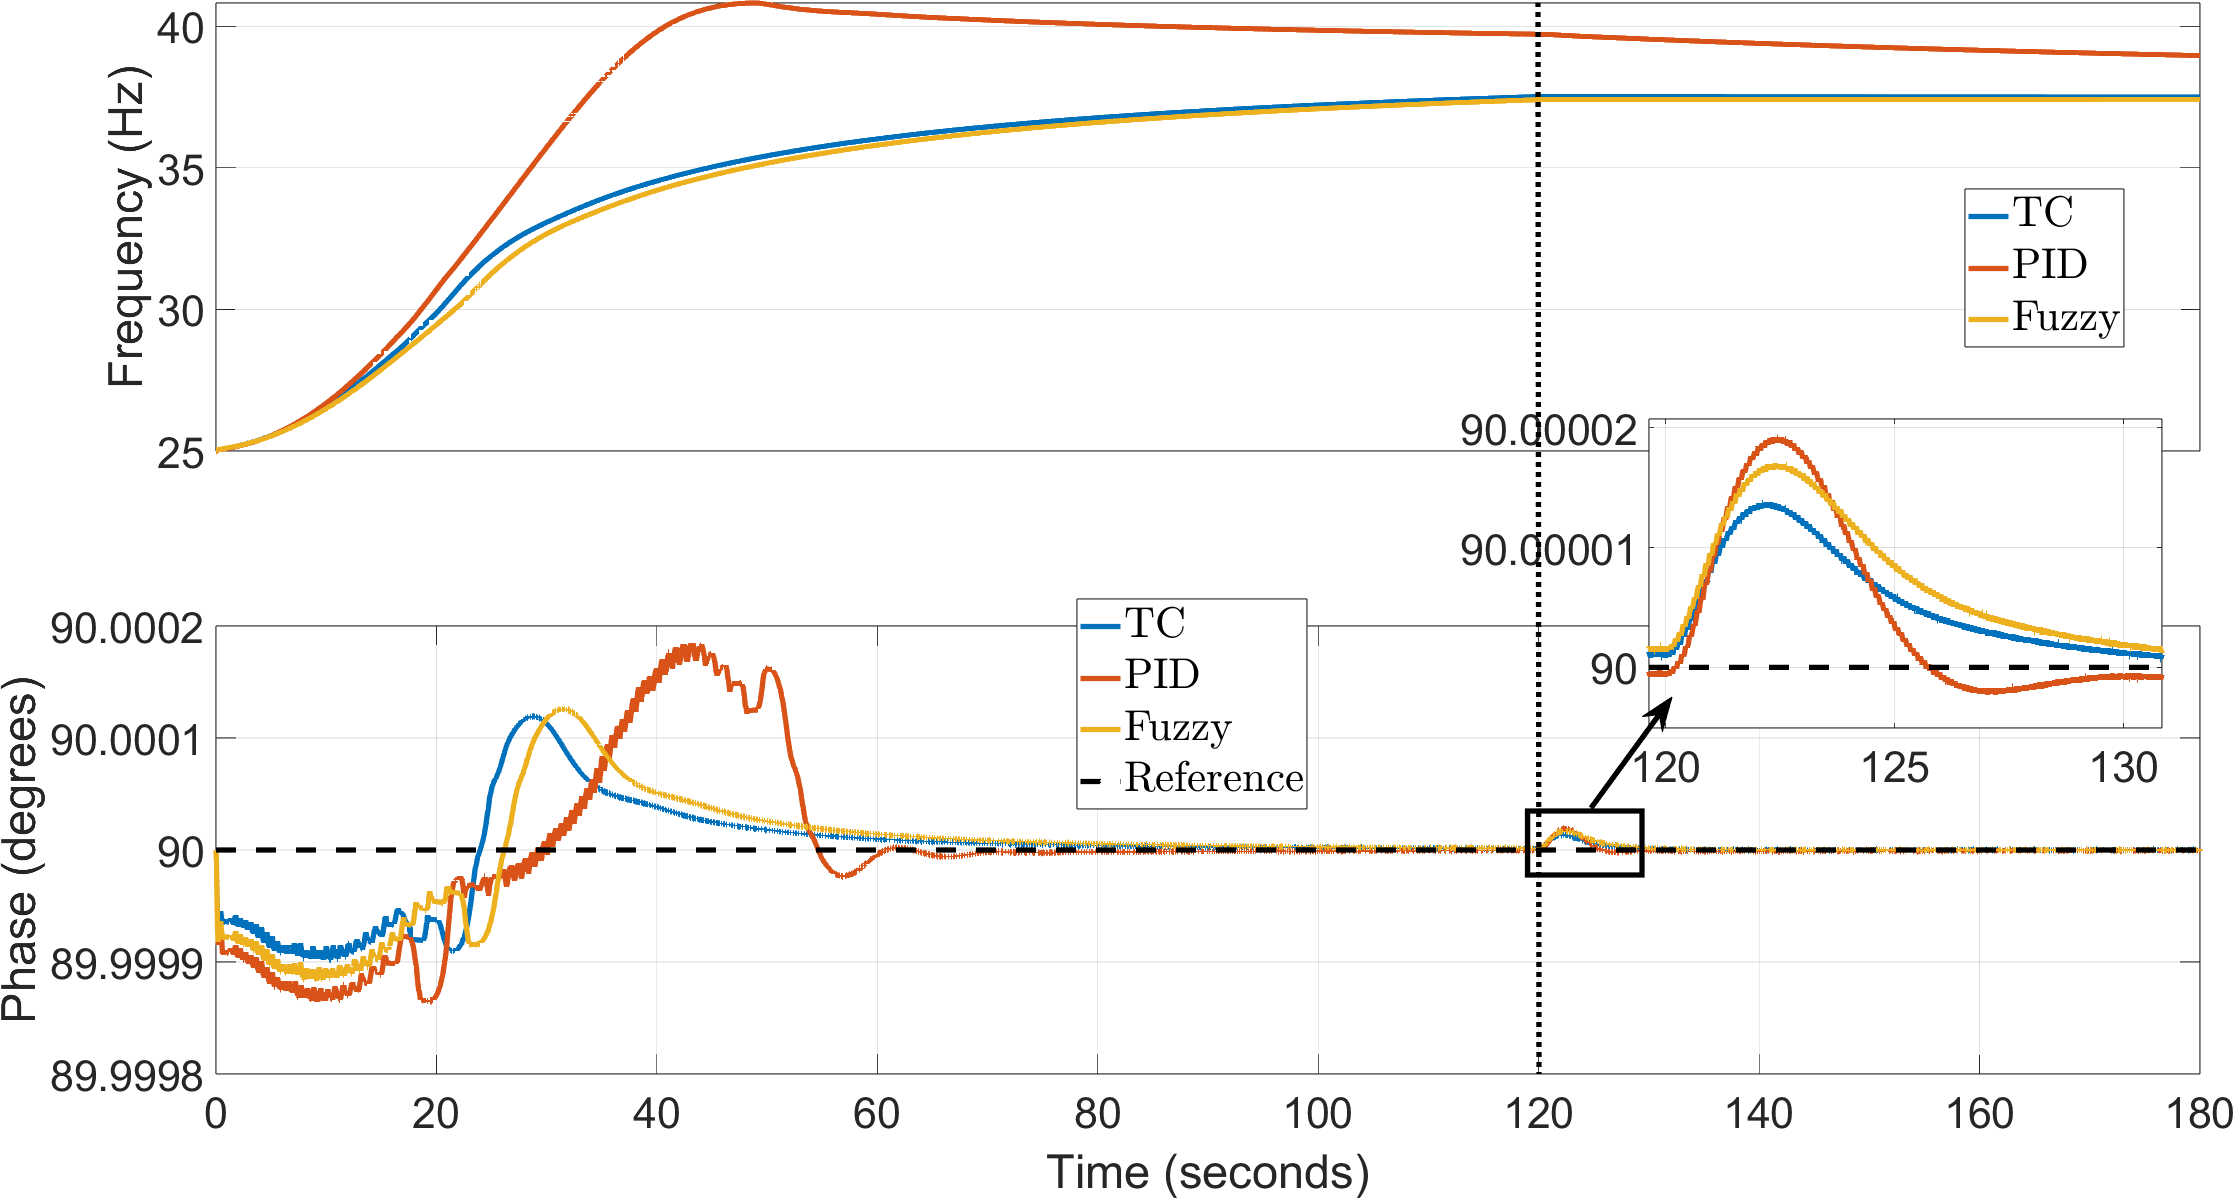
\includegraphics[width=\linewidth]{F_frequency_sim.png}
    \caption{Simulation: frequency and the phase ($k=256 \rightarrow 236$ N/m at t=120~s)}
    \label{F_sim_frequency}
\end{figure}

\begin{figure}
    \centering    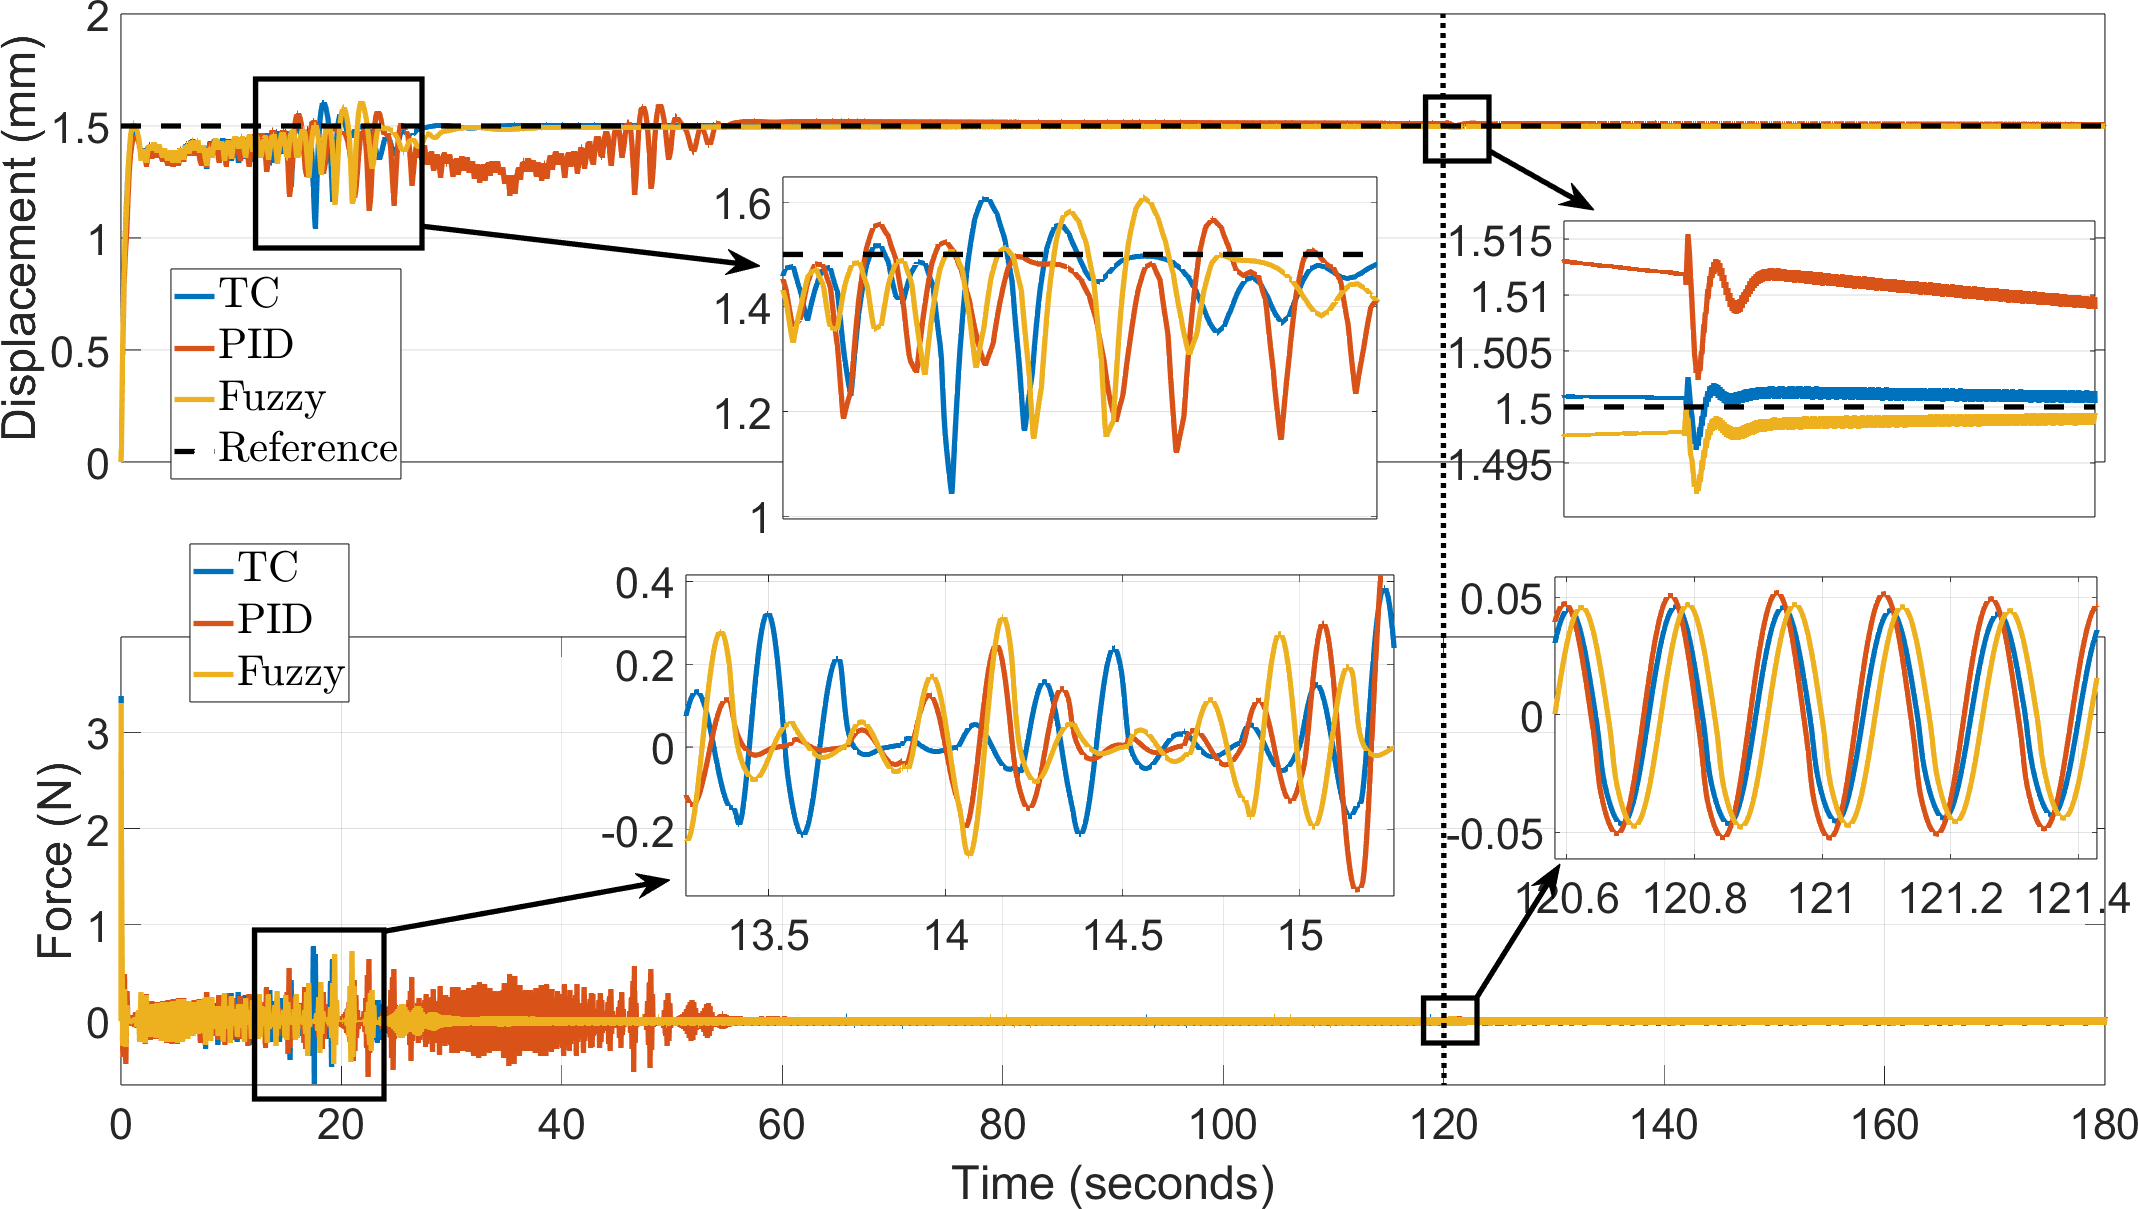
\includegraphics[width=\linewidth]{F_displacement_sim.png}
    \caption{Simulation: displacement and the force ($k=256 \rightarrow 236$ N/m at t=120~s)}
    \label{F_sim_displacement}
\end{figure}



\section{Practical experiments} \label{S_experiments}

The experimental setup is illustrated in \Cref{F_setup}. A specimen made of carbon fiber composite materials, with a theoretical resonance frequency of 39 Hz, is used. Two {\fontfamily{qcr}\selectfont B\&K 4502} accelerometers are mounted on the shaker and at the end of the specimen. The phase difference between these two measurements, along with the specimen's displacement, is provided to the controllers. Based on this input, the controllers compute the frequency and amplitude of the sinusoidal excitation force, which are then sent to a power amplifier. The amplified signals are applied to an {\fontfamily{qcr}\selectfont LDS V406} shaker, and the control loop is executed every second. All three controllers are implemented using {\fontfamily{qcr}\selectfont LabVIEW 2024 Q1} on a desktop computer equipped with an Intel Xeon E5-1607 CPU and 8 GB of RAM.


\begin{figure}
    \centering    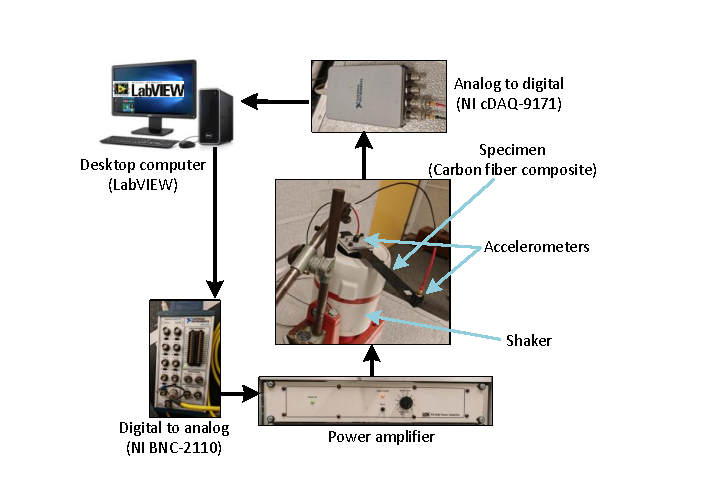
\includegraphics[width=\linewidth]{F_experiments.pdf}
    \caption{Experimental setup. Note that displacement is defined as the difference in amplitude between the positions measured by the installed accelerometers.
    }
    \label{F_setup}
\end{figure}

The parameters calculated in \Cref{T_parameters} are directly applied in the practical experiments without any retuning, to demonstrate the robustness of the controllers against perturbations present in a real setup. As in \Cref{S_simulations}, the first control objective is to track the desired displacement of 1.5~mm. However, the other objective is to track a desired phase of $89^\circ$, which differs from the $90^\circ$ used in the simulations. This adjustment is necessary because tracking exactly $90^\circ$ tends to induce instability; according to the Bode diagram in \Cref{F_Bode}, amplification is maximized at this phase, and with the relatively large sampling time of one second, the controllers cannot respond quickly enough to compensate for the resulting extreme displacement amplifications. In addition, due to this large sampling time, the TC cannot be implemented using explicit discretization, as it leads to numerical chattering. Instead, a deadbeat implementation is employed to address this issue (see \Cref{S_appendix} for the theory of deadbeat implementation). In a real fatigue testing facility, cracks typically appear in the specimen after a prolonged period (often several hours), causing changes in its resonance frequency. Under such conditions, the controllers must be robust enough to continue tracking the desired phase and adapt to the new resonance frequency.





The results of 100 seconds of experimental tests are presented in \Cref{F_phase,F_frequency,F_amplitude,F_amplitude_control_signal}. According to \Cref{F_phase}, while the TC implemented using the deadbeat scheme is free from chattering, the explicitly implemented TC suffers from significant chattering due to the discontinuous signum function $\sgn(\cdot)$ in its control law and the relatively large sampling time of one second (this issue is analysed in detail in \Cref{S_appendix}). The deadbeat-based TC demonstrates the fastest transient response and nearly zero steady-state error. In contrast, the PID controller exhibits large oscillations during the transient phase, which could lead to instability in other real-world scenarios involving such a multivariable system. Additionally, the fuzzy controller shows the slowest convergence in phase tracking. Furthermore, both the deadbeat TC and the PID controller achieve nearly zero steady-state tracking error, which is slightly better than the performance of the fuzzy controller. The frequencies computed by the controllers are shown in \Cref{F_frequency}, confirming the previous observations and demonstrating convergence around the theoretically calculated frequency of 39 Hz.

In addition to phase tracking, the other control objective is to maintain the displacement at 1.5~mm. As shown in \Cref{F_amplitude}, the TC implemented using the deadbeat scheme exhibits the fastest transient response and zero steady-state tracking error. Apart from the explicitly implemented TC, which suffers from chattering, all other controllers achieve zero steady-state error in displacement tracking. However, the PID controller shows a long convergence time, and the fuzzy controller exhibits significant displacement overshoots. These overshoots, as seen in \Cref{F_amplitude}, are particularly critical, making the fuzzy control strategy unsuitable for real fatigue testing. Displacement overshoots can lead to early specimen damage and result in noncompliance with testing standards.
These experimental results are obtained using the parameters tuned in \Cref{S_simulations}. While slight changes in parameters may affect the conclusions, the primary goal is to evaluate the robustness of the controllers when directly applying simulation-based tuning in real-world conditions. The amplitude of the excitation force $a$ generated by the controllers is shown in \Cref{F_amplitude_control_signal}. It is important to note that displacement is influenced by both the amplitude control signal $a$ and the frequency, due to the system’s multivariable characteristics. Moreover, it can again be observed that the explicitly implemented TC exhibits chattering in its amplitude control signal, in \Cref{F_amplitude_control_signal}, resulting in chattering in displacement tracking and making it unsuitable for practical applications with such a large sampling time of one second.
The quantified results corresponding to the experiments are given in \Cref{T_J_experiment}, indicating that the TC implemented based on the deadbeat method provides better transient performances in both phase and displacement tracking compared to the widely used PID controller.






\begin{figure}
    \centering    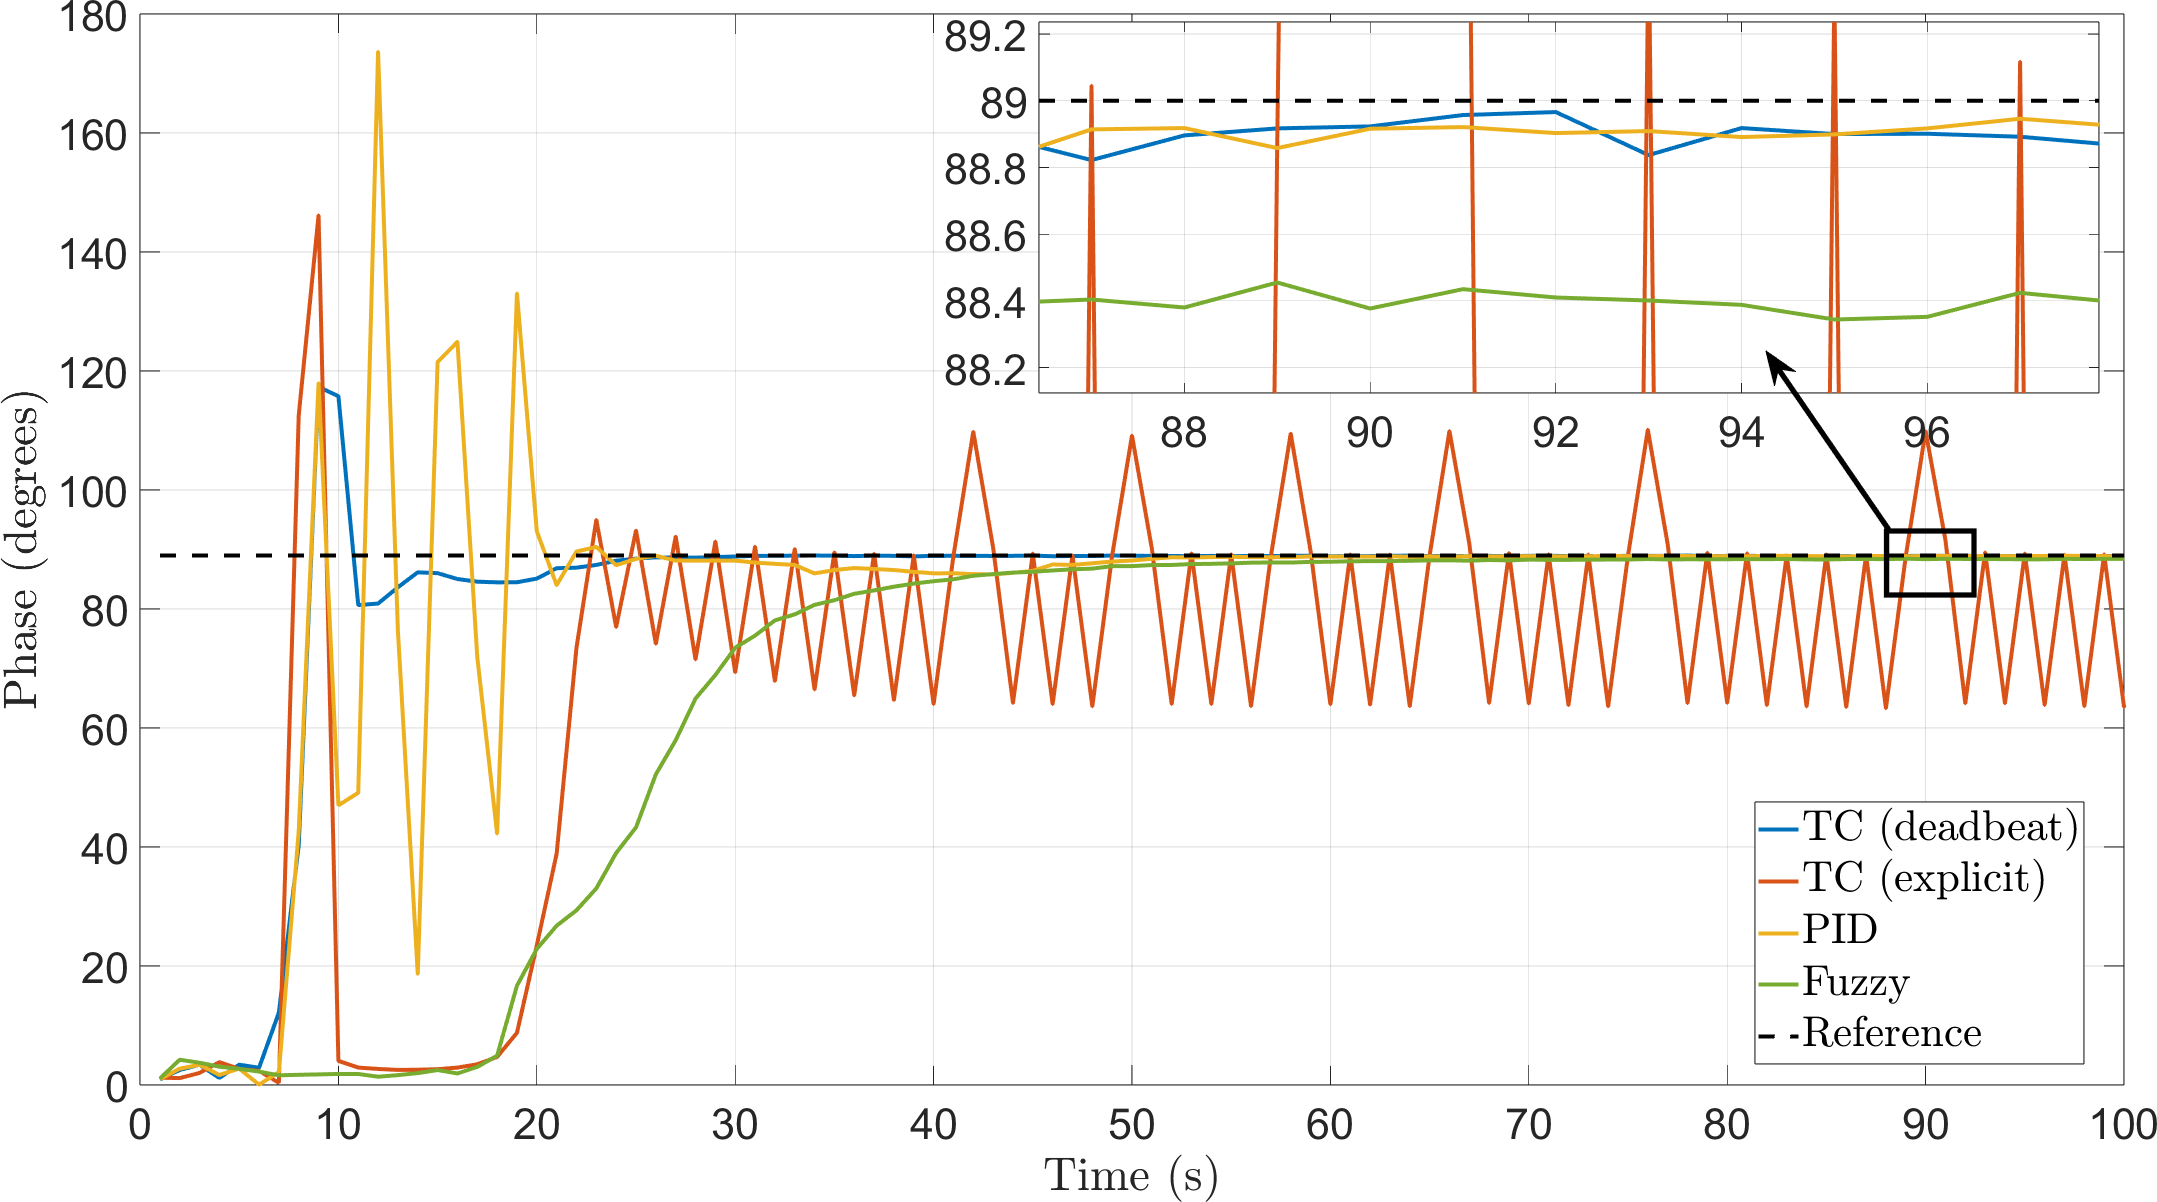
\includegraphics[width=\linewidth]{F_phase.png}
    \caption{Experiment: phase}
    \label{F_phase}
\end{figure}

\begin{figure}
    \centering    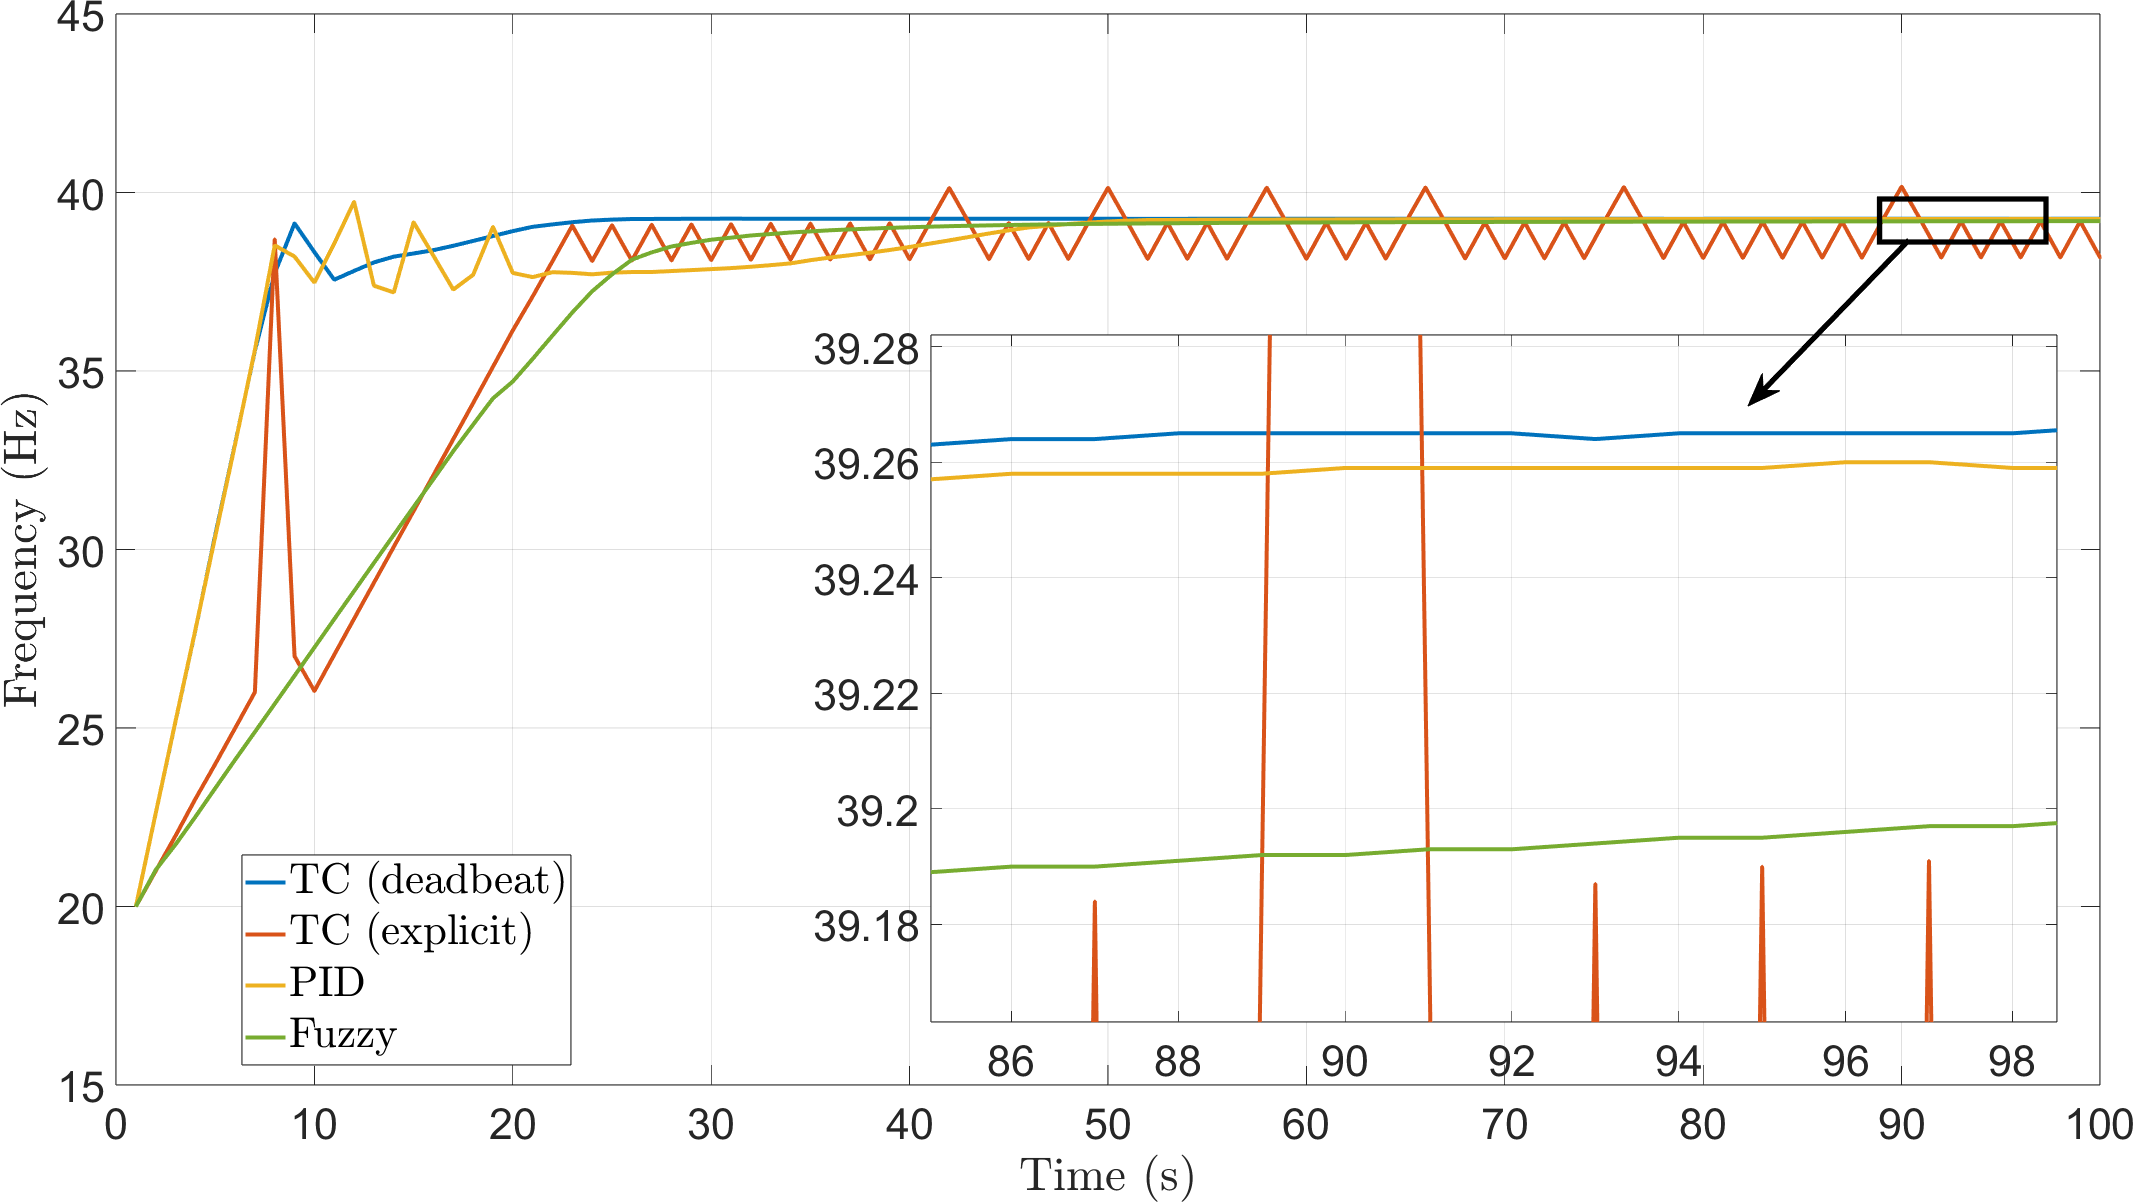
\includegraphics[width=\linewidth]{F_frequency.png}
    \caption{Experiment: frequency}
    \label{F_frequency}
\end{figure}


\begin{figure}
    \centering    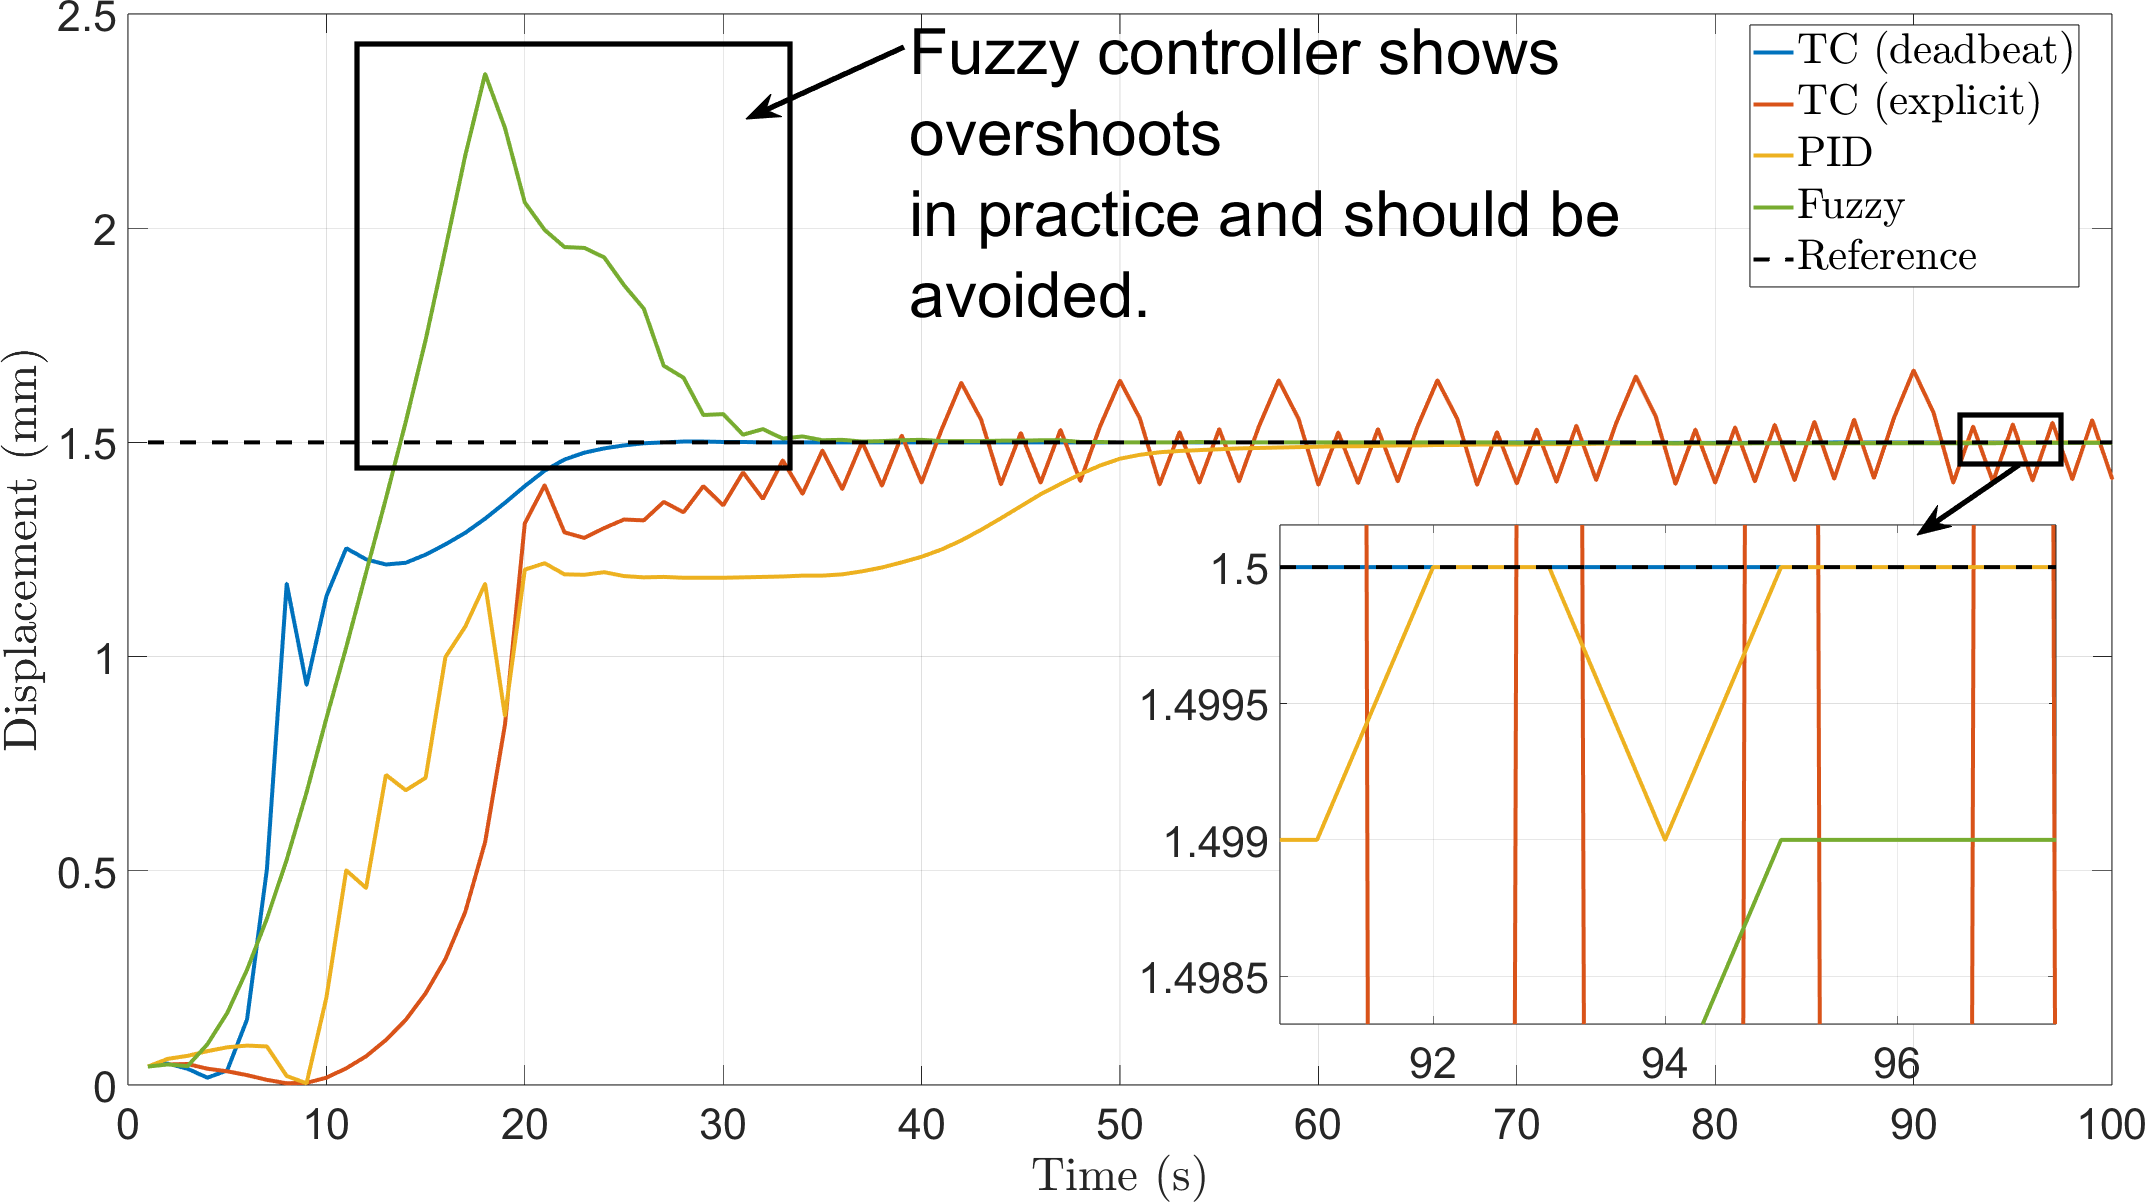
\includegraphics[width=\linewidth]{F_displacement.png}
    \caption{Experiment: displacement}
    \label{F_amplitude}
\end{figure}

\begin{figure}
    \centering    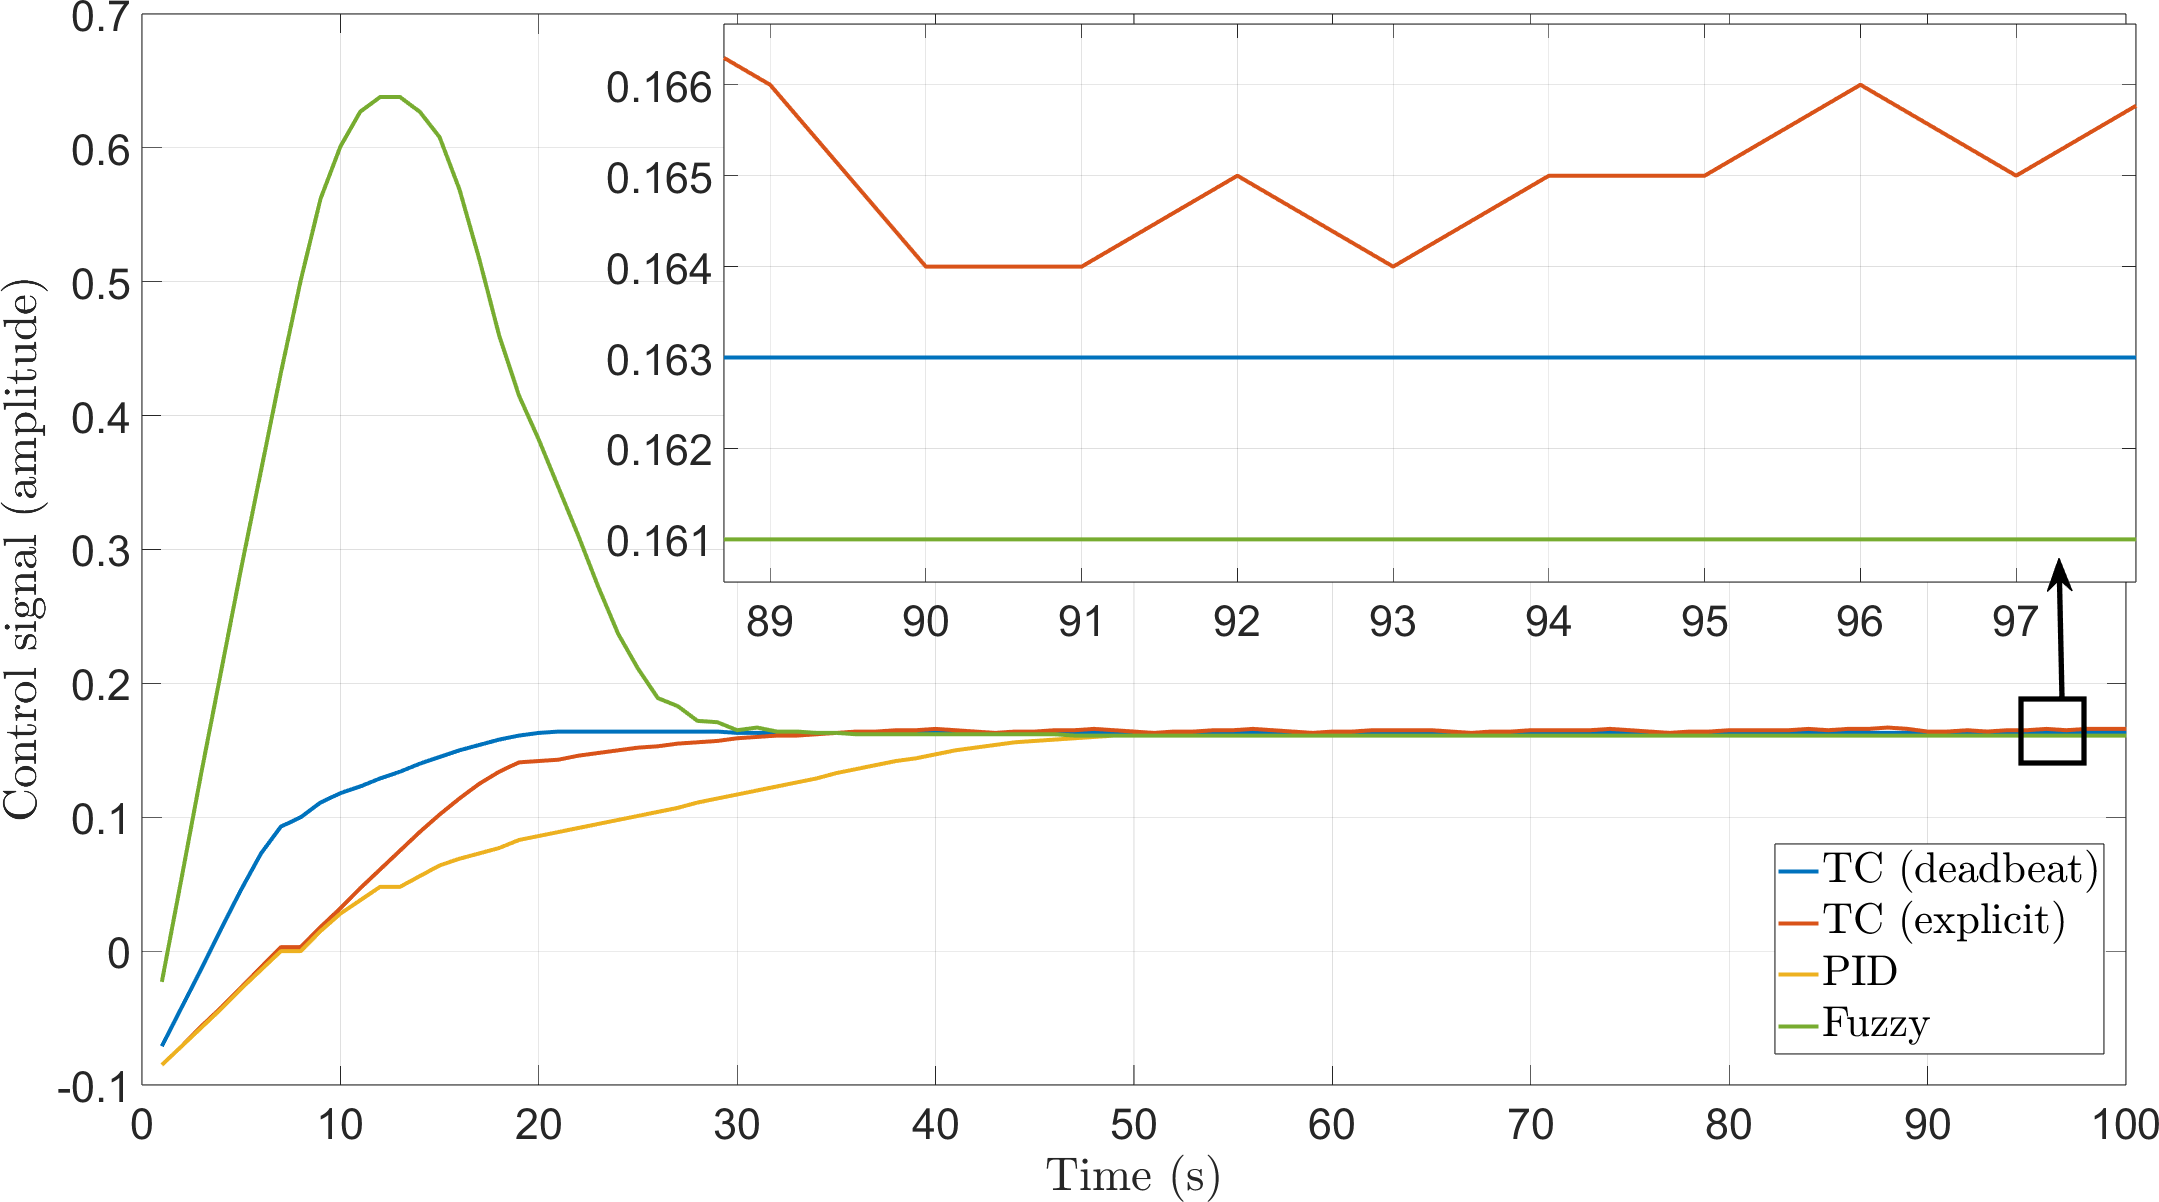
\includegraphics[width=\linewidth]{F_control_amplitude.png}
    \caption{Experiment: amplitude control signal}
    \label{F_amplitude_control_signal}
\end{figure}



\begin{table}
    \centering
    \begin{tabular}{|l|c|c|c|c|} \hline
       \cellcolor{gray}  &  TC (deadbeat) &  TC (explicit)   & PI & fuzzy   \\  \hline 
      $J_x$     & 3.8226    & 6.0040    &  5.2384   & 4.6702  \\  \hline 
      $J_\phi$  & 237.6890  & 403.2728  & 283.0377  & 444.3254  \\ \hline 
       $J$ &  241.5116      & 409.2768  &   288.2761 & 448.9956 \\ \hline 
    \end{tabular}
    \vspace{0.1cm}
    \caption{Experiment: displacement and phase tracking performances}
    \label{T_J_experiment}
\end{table}



\section{Conclusions} \label{S_conclusions}

This study explored the control design of fatigue testing machines—a topic that remains relatively underexplored. It began with a comprehensive tutorial reviewing the state of the art in controller design and implementation for fatigue testing systems. A control-oriented model of the system was then developed using identification methods, enabling the design of model-based controllers. This approach was necessary because classical modeling methods often produce models that are unsuitable for controller design.
A sliding-mode controller based on the twisting algorithm was designed to meet two primary control objectives: phase tracking and displacement tracking. Phase tracking is essential for maintaining the specimen at its resonance frequency, thereby reducing energy consumption. Displacement tracking ensures compliance with standards such as DIN 50100. Due to the relatively large experimental sampling time of one second, explicit discretization of the twisting controller led to chattering. To address this issue, a deadbeat implementation was developed and supported by mathematical theorems demonstrating chattering elimination and convergence. For comparison, two widely used control strategies—PID and fuzzy controllers—were also adapted and tuned through systematic numerical simulations.
All controllers, using the same gain values obtained from simulations, were implemented and tested on a real fatigue testing machine. Experimental results showed that the deadbeat-based twisting controller achieved slightly better transient and steady-state performance in both phase and displacement tracking. Apart from the explicitly implemented twisting controller, all control strategies provided acceptable tracking errors for both objectives. However, the fuzzy controller exhibited significant displacement overshoots, leading to noncompliance with standards and making it unsuitable for fatigue testing applications.
A key limitation observed during the experiments was the inability to maintain a 90° phase shift due to system instability. At this phase, the system gain increases sharply—as shown in the Bode diagram—and the controllers, constrained by the one-second sampling time, lack the responsiveness needed to maintain stability. Moreover, the system’s natural damping is minimized at 90°, making it impossible to reduce displacement amplitude. A potential solution for future studies is to adopt a multivariable control approach that introduces damping through the frequency control channel, effectively shifting the phase and stabilizing the displacement control channel.

\section*{Acknowledgments}

The authors gratefully acknowledge the support provided by Institut Carnot ARTS in France for this research.

\appendix[Deadbeat implementation of the twisting controller] \label{S_appendix}

As mentioned in \Cref{R_chattering}, for a small sampling time used in the numerical simulations, the twisting controller can be implemented using the explicit discretization. However, for the practical experiments, the sampling time was one second and the explicit discretization led to the chattering. The deadbeat implementation is explained here only for the phase tracking loop which can be extended to the phase tracking loop. Note that the deadbeat implementation is originally developed for another sliding-mode algorithm, namely, super-twisting algorithm \cite{MOJALLIZADEH_Franklin}, and is adopted for the twisting algorithm as follows. Consider again the nominal system's model \Cref{E_plant_identified_model} and the TC \Cref{E_TC} in the continuous-time setting: 
\begin{subequations}
  \begin{empheq}[left=\empheqlbrace]{align}
\dot{z}_1(t)&=z_2(t) \label{E_plant_identified_model_1a} \\
\dot{z}_2(t)&=pz_2+qu_1(t)  \label{E_plant_identified_model_2a} 
\\
u_1(t) &=  -\frac{p}{q}z_2 -b_1 \sgn(z_1) -b_2 \sgn(z_2). \label{E_TC_a}
  \end{empheq}
\label{E_plant_identified_modela}
\end{subequations}
Assuming that $qu=p z_2 +qu_1$, with the new control input $u$, \Cref{E_plant_identified_modela} can be rewritten as:
\begin{subequations}
  \begin{empheq}[left=\empheqlbrace]{align}
\dot{z}_1(t)&=z_2(t) \label{E_plant_identified_model_1a2} \\
\dot{z}_2(t)&=qu(t)  \label{E_plant_identified_model_2a2} 
\\
u(t) &=  -b_1 \sgn(z_1) -b_2 \sgn(z_2). \label{E_TC_a2}
  \end{empheq}
\label{E_plant_identified_modela2}
\end{subequations}
To implement the twisting control law \Cref{E_TC_a} on digital computers, a time-discretization must be employed. Explicit time-discretization of \Cref{E_plant_identified_modela2} reads as:
\begin{subequations}
  \begin{empheq}[left=\empheqlbrace]{align}
z_{1,k} &= h z_{2,k} + z_{1,k-1} \label{E_plant_identified_model_1a2_explicit} \\
z_{2,k} &=h q u_k + z_{2,k-1} , \label{E_plant_identified_model_2a2_explicit} 
\\
u_k &=  -b_1 \sgn(z_{1,k-1}) -b_2 \sgn(z_{2,k-1}), \label{E_TC_a2_explicit}
  \end{empheq}
\label{E_plant_identified_modela2_explicit}
\end{subequations}
where $h$ is the sampling time, and the subscript $k$ indicate the zero-order hold equivalent of a continuous-time variable such that $t=kh$. As reported in \cite{Huber2014,Huber2020,Xiong2020}, the explicit implementation of the twisting controller \Cref{E_plant_identified_modela2_explicit} lead to chattering and should be avoided. An alternative discretization is employed in this study as follows:
\begin{subequations}
  \begin{empheq}[left=\empheqlbrace]{align}
z_{1,k}&=h{z_{2,k-1}} + z_{1,k-1} \label{E_TC_plant_1_discrete_deadbeat} \\
z_{2,k} &=hu_k +z_{2,k-1} \label{E_TC_plant_2_discrete_deadbeat} \\
u_k    &\in -b_1  \sgnset(z_{1,k-1}) 
  -b_2\sgnsingle(z_{2,k-1}), \label{E_TC_discrete_control_deadbeat} 
  \end{empheq}
\label{E_TC_discrete_deadbeat}
\end{subequations}
where $\sgnset$ is the setvalued signum function defined in \Cref{E_sgn_function_set} and inclusion $\in$ is used to indicate the right-hand side of \Cref{E_TC_discrete_control_deadbeat} is setvalued.
\begin{equation}
\sgnset(s) \triangleq \left \{
    \begin{array}{lcl}
  -1   & \for & s\in \mathbb{R}^- \\
{[-1 , +1 ]}  & \for & s=  0 \\
   +1  & \for & s \in \mathbb{R}^+  . \\
    \end{array}
    \right.
    \label{E_sgn_function_set}
\end{equation}
Substituting \Cref{E_TC_discrete_control_deadbeat} into \Cref{E_TC_plant_2_discrete_deadbeat} gives the closed-loop equations as follows:
\begin{subequations}
  \begin{empheq}[left=\empheqlbrace]{align}
z_{1,k}&=h{z_{2,k-1}} + z_{1,k-1} \label{E_TC_plant_1_discrete_deadbeat_C1} \\
z_{2,k} &=-h b_1  \sgnset(z_{1,k-1}) 
  -h b_2\sgnsingle(z_{2,k-1}) + \notag \\
  & z_{2,k-1} .\label{E_TC_plant_2_discrete_deadbeat_C2}
  \end{empheq}
\label{E_TC_plant_2_discrete_deadbeat_C}
\end{subequations}
The term $\sgnset(z_{1,k-1})$ is a set which should be assigned to a single value to be able to synthesize the deadbeat control \Cref{E_TC_discrete_control_deadbeat}. This will be calculated through the selection procedure explained below. Substituting \Cref{E_TC_plant_2_discrete_deadbeat_C2} into \Cref{E_TC_plant_1_discrete_deadbeat_C1} gives:
\begin{equation}
\begin{array}{l}
z_{1,k} 
 \in -h^2b_1 \sgnset(z_{1,{k}})- 
h^2b_2\sgnsingle(z_{2,k-1}) \vspace{0.1cm} \\
+hz_{2,k-1} +z_{1,k-1} .
\end{array}
\label{E_closed_loop_x1}
\end{equation}
Following \cite{MOJALLIZADEH_Franklin}, and using \Cref{E_closed_loop_x1}, the selection of the term $\sgnset(z_{1,{k}})$, {\em i.e.}, $\lambda_k$ is calculated as follows:
\begin{equation}
\begin{array}{l}
\lambda_k=
\left \{
\begin{array}{lc}
q_{1,k}     &  \text{if} \hspace{0.3cm}  |q_{1,k}| \hspace{0.1cm} \text{and} \hspace{0.1cm} |q_{2,k}|<1   \\
 \sgnsingle(z_{1,k-1})    &   \text{else},
\end{array}
\right.  \vspace{0.2cm} \\ 
q_{1,k}=\frac{-h^2b_2\sgnsingle(z_{2,k-1})+hz_{2,k-1}+z_{1,k-1}}{h^2b_1} , \vspace{0.2cm} \\ 
q_{2,k}=\frac{-h^2b_2\sgnsingle(z_{1,k-1}/h)-z_{1,k-1}}{h^2b_1} .
\end{array}
\label{E_q}
\end{equation}


\begin{equation}
u_k = -b_1  \lambda_{k}
  -b_2\sgnsingle(z_{2,k-1}).\label{E_TC_discrete_control_explicit_solved} 
\end{equation}

\begin{lemma} \label{Lemma_invariant}
The origin $(z_{1,k} , z_{2,k})=(0,0)$ is the invariance equilibrium point of the closed-loop system in the presence of the control law  \Cref{E_TC_discrete_control_explicit_solved} and the plant \Cref{E_TC_plant_1_discrete_deadbeat,E_TC_plant_2_discrete_deadbeat}.

\noindent \textbf{Proof.}  For $(z_{1,k-1} , z_{2,k-1})=(0,0)$, from \Cref{E_TC_discrete_control_explicit_solved,E_q}, one has $u_k=0$.
Substituting these values into \Cref{E_TC_plant_1_discrete_deadbeat,E_TC_plant_2_discrete_deadbeat} gives:
\begin{subequations}
  \begin{empheq}[left=\empheqlbrace]{align}
z_{1,k}&=0
\label{E_TC_closed_loop_discrete1_proof} \\
z_{2,k} &=0
.\label{E_TC_closed_loop_discrete2_proof} 
  \end{empheq}
\label{E_TC_closed_loop_discrete_proof}
\end{subequations}
Hence, once the system arrives at the origin, it stays there, indicating that the origin is the invariance equilibrium point of the closed-loop system \Cref{E_TC_plant_1_discrete_deadbeat,E_TC_plant_2_discrete_deadbeat} under the control law \Cref{E_TC_discrete_control_explicit_solved,E_q}. $\blacksquare$
\end{lemma}


\begin{theorem} \label{Theorem_nominal}
    The unperturbed second-order system \Cref{E_TC_plant_1_discrete_deadbeat,E_TC_plant_2_discrete_deadbeat} under the control law \Cref{E_TC_discrete_control_explicit_solved,E_q} converges to the origin.
\end{theorem}
\noindent \textbf{Proof.} 
Substituting \Cref{E_TC_discrete_control_explicit_solved} into \Cref{E_TC_plant_1_discrete_deadbeat,E_TC_plant_2_discrete_deadbeat}, the closed-loop equations turn into:
\begin{subequations}
  \begin{empheq} [left=\empheqlbrace]{align}
z_{1,k}&=hz_{2,k} + z_{1,k-1} \label{E_TC_closed_loop_discrete1_lambda} \\
z_{2,k} & = -hb_1  \lambda_k- hb_2\sgnsingle(z_{2,k-1}) +z_{2,k-1} .\label{E_TC_closed_loop_discrete2_lambda} 
  \end{empheq}
\label{E_TC_closed_loop_discrete_lambda}
\end{subequations}
The convergence will be studied for two partitioning regions defined by ($|q_{1,k}|< 1$ and $|q_{2,k}|<1$) and ($|q_{1,k}|\geq 1$ or $|q_{2,k}|\geq 1$) as follows:
\begin{itemize}


    \item $\boldsymbol{|q_{1,k}|< 1$ and $|q_{2,k}|<1}$:
In this case, one has
\begin{equation}
\lambda_k=\frac{-h^2b_2\sgnsingle(z_{2,k-1})+hz_{2,k-1}+z_{1,k-1}}{h^2b_1} .
\label{E_deadbeat_term_nosat}
\end{equation}
Inserting \Cref{E_deadbeat_term_nosat} into \Cref{E_TC_closed_loop_discrete_lambda} gives:
\begin{subequations}
  \begin{empheq}[left=\empheqlbrace]{align}
z_{1,k}&=hz_{2,k} + z_{1,k-1}=0 \label{E_TC_closed_loop_final_1} \\
z_{2,k} & = -\frac{z_{1,k-1}}{h}.\label{E_TC_closed_loop_final_2}
  \end{empheq}
\label{E_TC_closed_loop_final}
\end{subequations}
It means that once the system arrives in this region, just one step after, at $k$, one has $z_{1,k}=0$ and $z_{2,k}=\frac{z_{1,k-1}}{h}$. In this case, substituting these values into $q_{1,k}$ and $q_{2,k}$ in \Cref{E_qq} gives:
\begin{equation}
\begin{array}{l}
q_{2,k+1}=\frac{-h^2b_2\sgnsingle(z_{1,k}/h)-z_{1,k}}{h^2b_1} =0.
\vspace{0.2cm} \\
q_{1,k+1}=\frac{-h^2b_2\sgnsingle(z_{2,k})+hz_{2,k}+z_{1,k}}{h^2b_1} =  \frac{-h^2b_2\sgnsingle(z_{1,k}/h)}{h^2b_1} \vspace{0.2cm}\\
=\frac{-h^2b_2\sgnsingle(z_{1,k}/h)-z_{1,k}}{h^2b_1}=q_{2,k}.
\end{array}
\end{equation}

It can be seen that $q_{2,k+1}=0$ which clearly satisfies $|q_{2,k+1}|<1$. On the other hand, $q_{1,k+1}=q_{2,k}$. Since $|q_{2,k}|<1$ already holds, one has $|q_{1,k+1}|<1$. With $|q_{1,k+1}|<1$  and $|q_{2,k+1}|<1$, the deadbeat mechanism will be reactivated at the next time step $k+1$. Repeating the same procedure gives:
\begin{subequations}
  \begin{empheq}[left=\empheqlbrace]{align}
z_{1,k}&=hz_{2,k} + z_{1,k-1}=0 \label{E_TC_closed_loop_final_123} \\
z_{2,k} & = -\frac{z_{1,k-1}}{h}=0,\label{E_TC_closed_loop_final_223}
  \end{empheq}
\label{E_TC_closed_loop_final_23}
\end{subequations}
which indicates the convergence to the origin. In addition, according to \Cref{Lemma_invariant}, since the origin is the invariance equilibrium point of the closed-loop system, the system stays at the origin after that. 

  \item $\boldsymbol{|q_{1,k}|\geq 1$ or $|q_{2,k}|\geq 1}$:   From \Cref{E_q}, in this case, one has $\lambda_k=\sgnsingle(z_{1,k-1})$. Therefore,  \Cref{E_TC_discrete_control_explicit_solved} becomes a classic explicit discretization of the twisting controller, and the problem turns into stability analysis of the explicit TC \Cref{E_plant_identified_modela2_explicit}. Unfortunately, the convergence of the explicitly implemented TC \Cref{E_plant_identified_modela2_explicit} has not yet been addressed directly. Assuming that the explicitly implemented TC \Cref{E_plant_identified_modela2_explicit} follows its continuous-time \Cref{E_TC} behavior in this region, the stability theorems presented for the continuous-time TC can be used for this purpose (see \cite{Santiesteban_twisting,POLYAKOV_twisting,Orlov_twisting,UTKIN_twisting_stablity,Oza_twisting}) to show the state variables $z_{1,k-1}$ and $z_{2,k-1}$ tend to the origin for a sufficiently large $k$, {\em i.e.}, $z_{1,k-1} \rightarrow 0$ and $z_{2,k-1} \rightarrow 0$ as $k \rightarrow \infty$. Substituting these values into $q_{1,k}$ and $q_{2,k}$
 defined in \Cref{E_q} gives $q_{1,k} \rightarrow 0$ and $q_{2,k} \rightarrow 0$ leading to ($|q_{1,k}|< 1$ and $|q_{2,k}|<1$) (note that $b_1>b_2>0$).
It indicates that for a sufficiently large $k$, the system enters the region defined in the first case, leading to the activation of the deadbeat control, which was studied in the previous case. It should be noted that such a fact, {\em i.e.}, converging the explicit discretization of the TC, in this region to its continuous-time behavior, has not yet been studied, and the author believes that this deserves revisited in future studies. 
    $\blacksquare$
\end{itemize}





%{\appendices
%\section*{Proof of the First Zonklar Equation}
%Appendix one text goes here.
% You can choose not to have a title for an appendix if you want by leaving the argument blank
%\section*{Proof of the Second Zonklar Equation}
%Appendix two text goes here.}

\bibliographystyle{IEEEtran}
\bibliography{Mybib}



\newpage

\section{Biography Section}
 

\begin{IEEEbiography}[{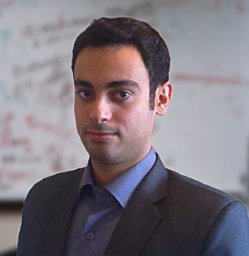
\includegraphics[width=1in,height=1.25in,clip,keepaspectratio]{F_mojalli.jpg}}]{Mohammad Rasool MOJALLIZADEH} was born in Isfahan, Iran, in 1988. He
received the Ph.D. degree in control engineering from the University of Tabriz, Iran, in 2017, with the highest academic distinction of Excellence. He subsequently joined INRIA, France, as a postdoctoral researcher on the ANR Digitslid and IRT Nanoelec projects until 2022. In 2022, he worked as a research engineer at Centrale Nantes, France, contributing to several national and European projects, including the H2020 project FLOATECH and the ANR CREATIF project. Since 2024, he has been a lecturer-researcher at the Arts et Métiers Institute of Technology.
\end{IEEEbiography}

\vspace{11pt}

\begin{IEEEbiography}[{
\includegraphics[width=1in,height=1.45in,clip,keepaspectratio]{Etienne.jpg}}]{Etienne PESSARD} was born in France. He received the Ph.D. degree in Mechanics and Materials in 2009. He then worked as a lecturer and researcher for 10 years, during which he contributed to numerous projects, including FUI QUAUSI, ANR DEFISURF, IRT Jules Verne projects FATAL and FASICOM. In parallel, he co-supervised several industrial Ph.D. theses focused on the fatigue resistance of metals. After a one-year experience as a visiting professor at École Polytechnique de Montréal, his research activities shifted toward vibrational fatigue testing using shakers. Since 2024, he has been a Professor at the Arts et Métiers Institute of Technology.

\end{IEEEbiography}

\vspace{11pt}

\begin{IEEEbiography}[{
\includegraphics[width=1in,height=1.25in,clip,keepaspectratio]{avatar.png}}]{Benoît PICHEREAU}

\end{IEEEbiography}

\vspace{11pt}

\bf{If you will not include a photo:}\vspace{-33pt}
\begin{IEEEbiographynophoto}{John Doe}
Use $\backslash${\tt{begin\{IEEEbiographynophoto\}}} and the author name as the argument followed by the biography text.
\end{IEEEbiographynophoto}




\vfill

\end{document}


